\documentstyle[epic,eepic,graphicx,tabularx,mathtools,cite,subfig,caption,appendix,algorithm,algorithmicx,algpseudocode,amssymb,listings,color,afterpage]{poly3}

%\mathindent 0pt
\input{preamble}
\input{epsf}

% Override the double parenthesis
\newtagform{defaultoveride}{}{}
\usetagform{defaultoveride}


%%%%%%%%%%%%%%%%%%%%%%%%%%%%%%%%%%%%%%%%%%%%%%%%%%%
\renewcommand{\baselinestretch}{1.6}
\newtheorem{theorem}{Theorem}[chapter]
\newcommand{\btheorem}{\begin{theorem}\rm}
\newcommand{\etheorem}{$\diamond$\end{theorem}}
\newtheorem{definition}{Definition}[chapter]
\newcommand{\bdefn}{\begin{definition}\rm}
\newcommand{\edefn}{\end{definition}}
\newtheorem{lemma}{Lemma}[chapter]
\newtheorem{remark}{Remark}[chapter]
\newcommand{\bremark}{\begin{remark}\rm}
\newcommand{\eremark}{\end{remark}}
\newtheorem{example}{Example}[chapter]
\newcommand{\bexample}{\begin{example}\rm}
\newcommand{\eexample}{\end{example}}
\newtheorem{assumption}{Assumption}[chapter]
\newcommand{\bassump}{\begin{assumption}\rm}
\newcommand{\eassump}{\end{assumption}}
\begin{document}
\title{DESIGN AND CONTROL OF THE BLUEFOOT PLATFORM :\\A MULTI-TERRAIN QUADRUPED ROBOT}
\author{Brian Cairl}
\date{May, 2015}
\committee{1}

\mstitlepage
\topmargin=0.4in
\textwidth=6.0in
\textheight=9.0in


%%%%%%%%%%%%%%%%%%%%%%%%%%%%%%%%%%%%%%%%%%%%%%%%%%%



%%%%%%%%%%%%%%%%%%%%%%%%%%%%%%%%%%%%%%%%%%%%%%%%%%%
\setcounter{page}{1}
\pagenumbering{roman}
\chapter*{VITA}
	\vitaentry{Mar 23, 1992}{Born}
	\vitaentry{Sep, 2010}{Entered the NYU Polytechnic School of Engineering as a Mechanical Engineering major and an Honors student.}
	%\vitaentry{Jan, 2012}{Switched to an Electrical Engineering major. Registered as a BS/MS student.}
	%\vitaentry{May, 2012}{Entered the Controls/Robotics Research Laboratory as an undergraduate researcher. Began formal design of BlueFoot's predecessor, the GreenFoot Platform.}
	\vitaentry{Jun, 2012}{Completed a minor in Mechanical Engineering.}
	%\vitaentry{Jan, 2013}{Completed undergraduate Senior Design I under the advisement of Professor Farshad Khorrami.}
	\vitaentry{Oct, 2014}{Submitted a paper to the 2015 International Conference on Robotics and Automation (ICRA) summarizing the design and control of the BlueFoot platform .}
	\vitaentry{Mar, 2015}{Submitted a paper to the 2015 International Conference on Intelligent Robots and Systems (IROS) on a NARX Neural Network trunk leveling controller for legged robots .}
	%\vitaentry{May, 2013}{Admitted into the 2013 NYU Undergraduate Summer Research program under the advisement of Professor Farshad Khorrami. Began formal design of the BlueFoot Platform.}
	%\vitaentry{May, 2014}{Admitted into the 2014 NYU Undergraduate Summer Research program under the advisement of Professor Farshad Khorrami.}
	%\vitaentry{Sep-Oct, 2014}{Wrote a paper on the design and preliminary control of the BlueFoot Platform, which was submitted to ICRA2015. }
	%\vitaentry{Feb-Mar, 2014}{Wrote a paper on the neural-network based platform-leveling control of legged platforms, which was submitted to IROS2015.}
	\vitaentry{Apr, 2015}{Admitted to the  NYU Polytechnic School of Engineering as PhD Fellow under the advisement of Professor Farshad Khorrami.}
\include{publications}
\clearpage
\vspace*{\fill}
	\begin{center}
		\begin{minipage}{\textwidth}
			\hspace{5mm} 
			I would like to thank Professor Farshad Khorrami for his advisement throughout the course of this project, as well as for teaching me various elements of controls and robotics knowledge necessary for completing the work I have done up to this point. Professor Khorrami has helped guide me toward learning a set of skills and a base of knowledge which will be invaluable to my future work. I also thank Professor Khorrami for all the time he spent helping me to revise papers and discuss the different portions of my project with me. My time under his advisement has given me a wealth of insight about controls, robotics, research and scientific report writing in the academic setting.
			
			\vspace{5mm}
			\hspace{5mm} 
			I would also like to thank Dr. Krishnamurthy for his guidance in various implementation matters, including with matters of programming and discussing solutions to particular problems which were faced during the course of my work. Additionally, I would like to thank my colleague Griswald Brooks for countless instances of assistance with hardware-related matters during the design and construction of my robot. 
		\end{minipage}
	\end{center}
\vfill % equivalent to \vspace{\fill}
\clearpage

\clearpage
\vspace*{\fill}
	\begin{center}
		\begin{minipage}{\textwidth}
		\emph{
			I would like to dedicate this work to my loving mother, father, brother and grandparents for thier love and support through all my endeavors. 
		}
		\end{minipage}
	\end{center}
\vfill % equivalent to \vspace{\fill}
\clearpage
{\msabstract{Dr. Farshad Khorrami}}
{
	This thesis presents the development and control of a small-scale quadruped robot platform with 16 actuated degrees-of-freedom, named ``BlueFoot." The BlueFoot platform has been developed for the purpose of studying multi-terrain navigation and gait control in concert with full-body actuation, which may be used for reorienting payloads (\EG laser distance sensor and vision-sensor peripherals). This thesis will detail the design of the BlueFoot platform and its hardware sub-systems; an in-depth analysis of the system's kinematic model and robot dynamics; core Central-Pattern Generator (CPG) based gaiting algorithms introducing reflexive, feedback-driven mechanisms; and a unique foot placement and Zero-Moment Point (ZMP) posture controller based on a virtual force model and a posture feedback loop utilizing inertial measurements. %Lastly, this paper will include results from an object tracking task performed by the BlueFoot platform which utilizes a full-body actuation controller to track a moving target object through a combination of body pitch and roll adjustments, and omni-directional gaiting. 


	In addition, this thesis offers a method for attaining constant orientation of the trunk of a multi-legged (here a quadruped) robot in the presence of disturbances due to feet impact with the ground. This is significant when payloads (such as cameras, optical systems, armaments) are carried by the robot.  The trunk is stabilized by the utilization of an on-line learning method to actively correct the open-loop gait generated by a CPG or a limit-cycle method. The learning method is based on a Nonlinear Autoregressive Neural Network with Exogenous inputs (NARX-NN)-- a recurrent neural network architecture typically utilized for modeling nonlinear difference systems. A supervised learning approach is used to train the NARX-NN. 
	%The input to the neural network includes states of the robot legs, trunk attitude and attitude rates, and feet contact forces. The neural network is used to generate the total torque imparted on the robot. This approach allows on-line learning of the internal forces and disturbances due to various effects to be estimated/learned with the neural network for implementation in an inverse dynamics/computed torque controller. The controller is utilized to achieve a stable trunk (\IE a constant orientation of the trunk). 
	The efficacy of the proposed approach is shown in detailed simulation studies of a quadruped robot. 

	Lastly, this thesis will present several algorithms related to navigation control, terrain modeling, and rough-terrain gait planning. In particular, algorithms for surface reconstruction and foothold planning over uneven terrain will be integral components for future developments related to the BlueFoot project. Results from simulations and actual robot trials will be presented to demonstrate the performance of these control strategies. 
\clearpage}
{\endmsabstract}

\normalsize
\tableofcontents
\listoffigures
\listoftables
\newpage
\setcounter{page}{1}
\pagenumbering{arabic}
%%%%%%%%%%%%%%%%%%%%%%%%%%%%%%%%%%%%%%%%%%%%%%%%%%%
	%%%%%%%%%%%%%%%%%%%%%%%%%%%%%%%%%%%%%%%%%%%%%%%%%%%%%%%%%%%%%%%%%%%%%%%%%%%%%%%%%%
%%% Introduction
%%%%%%%%%%%%%%%%%%%%%%%%%%%%%%%%%%%%%%%%%%%%%%%%%%%%%%%%%%%%%%%%%%%%%%%%%%%%%%%%%%
\chapter{Introduction}
	\label{ch::introduction}
	
	\begin{figure}[h!]
		\centering
		\fbox{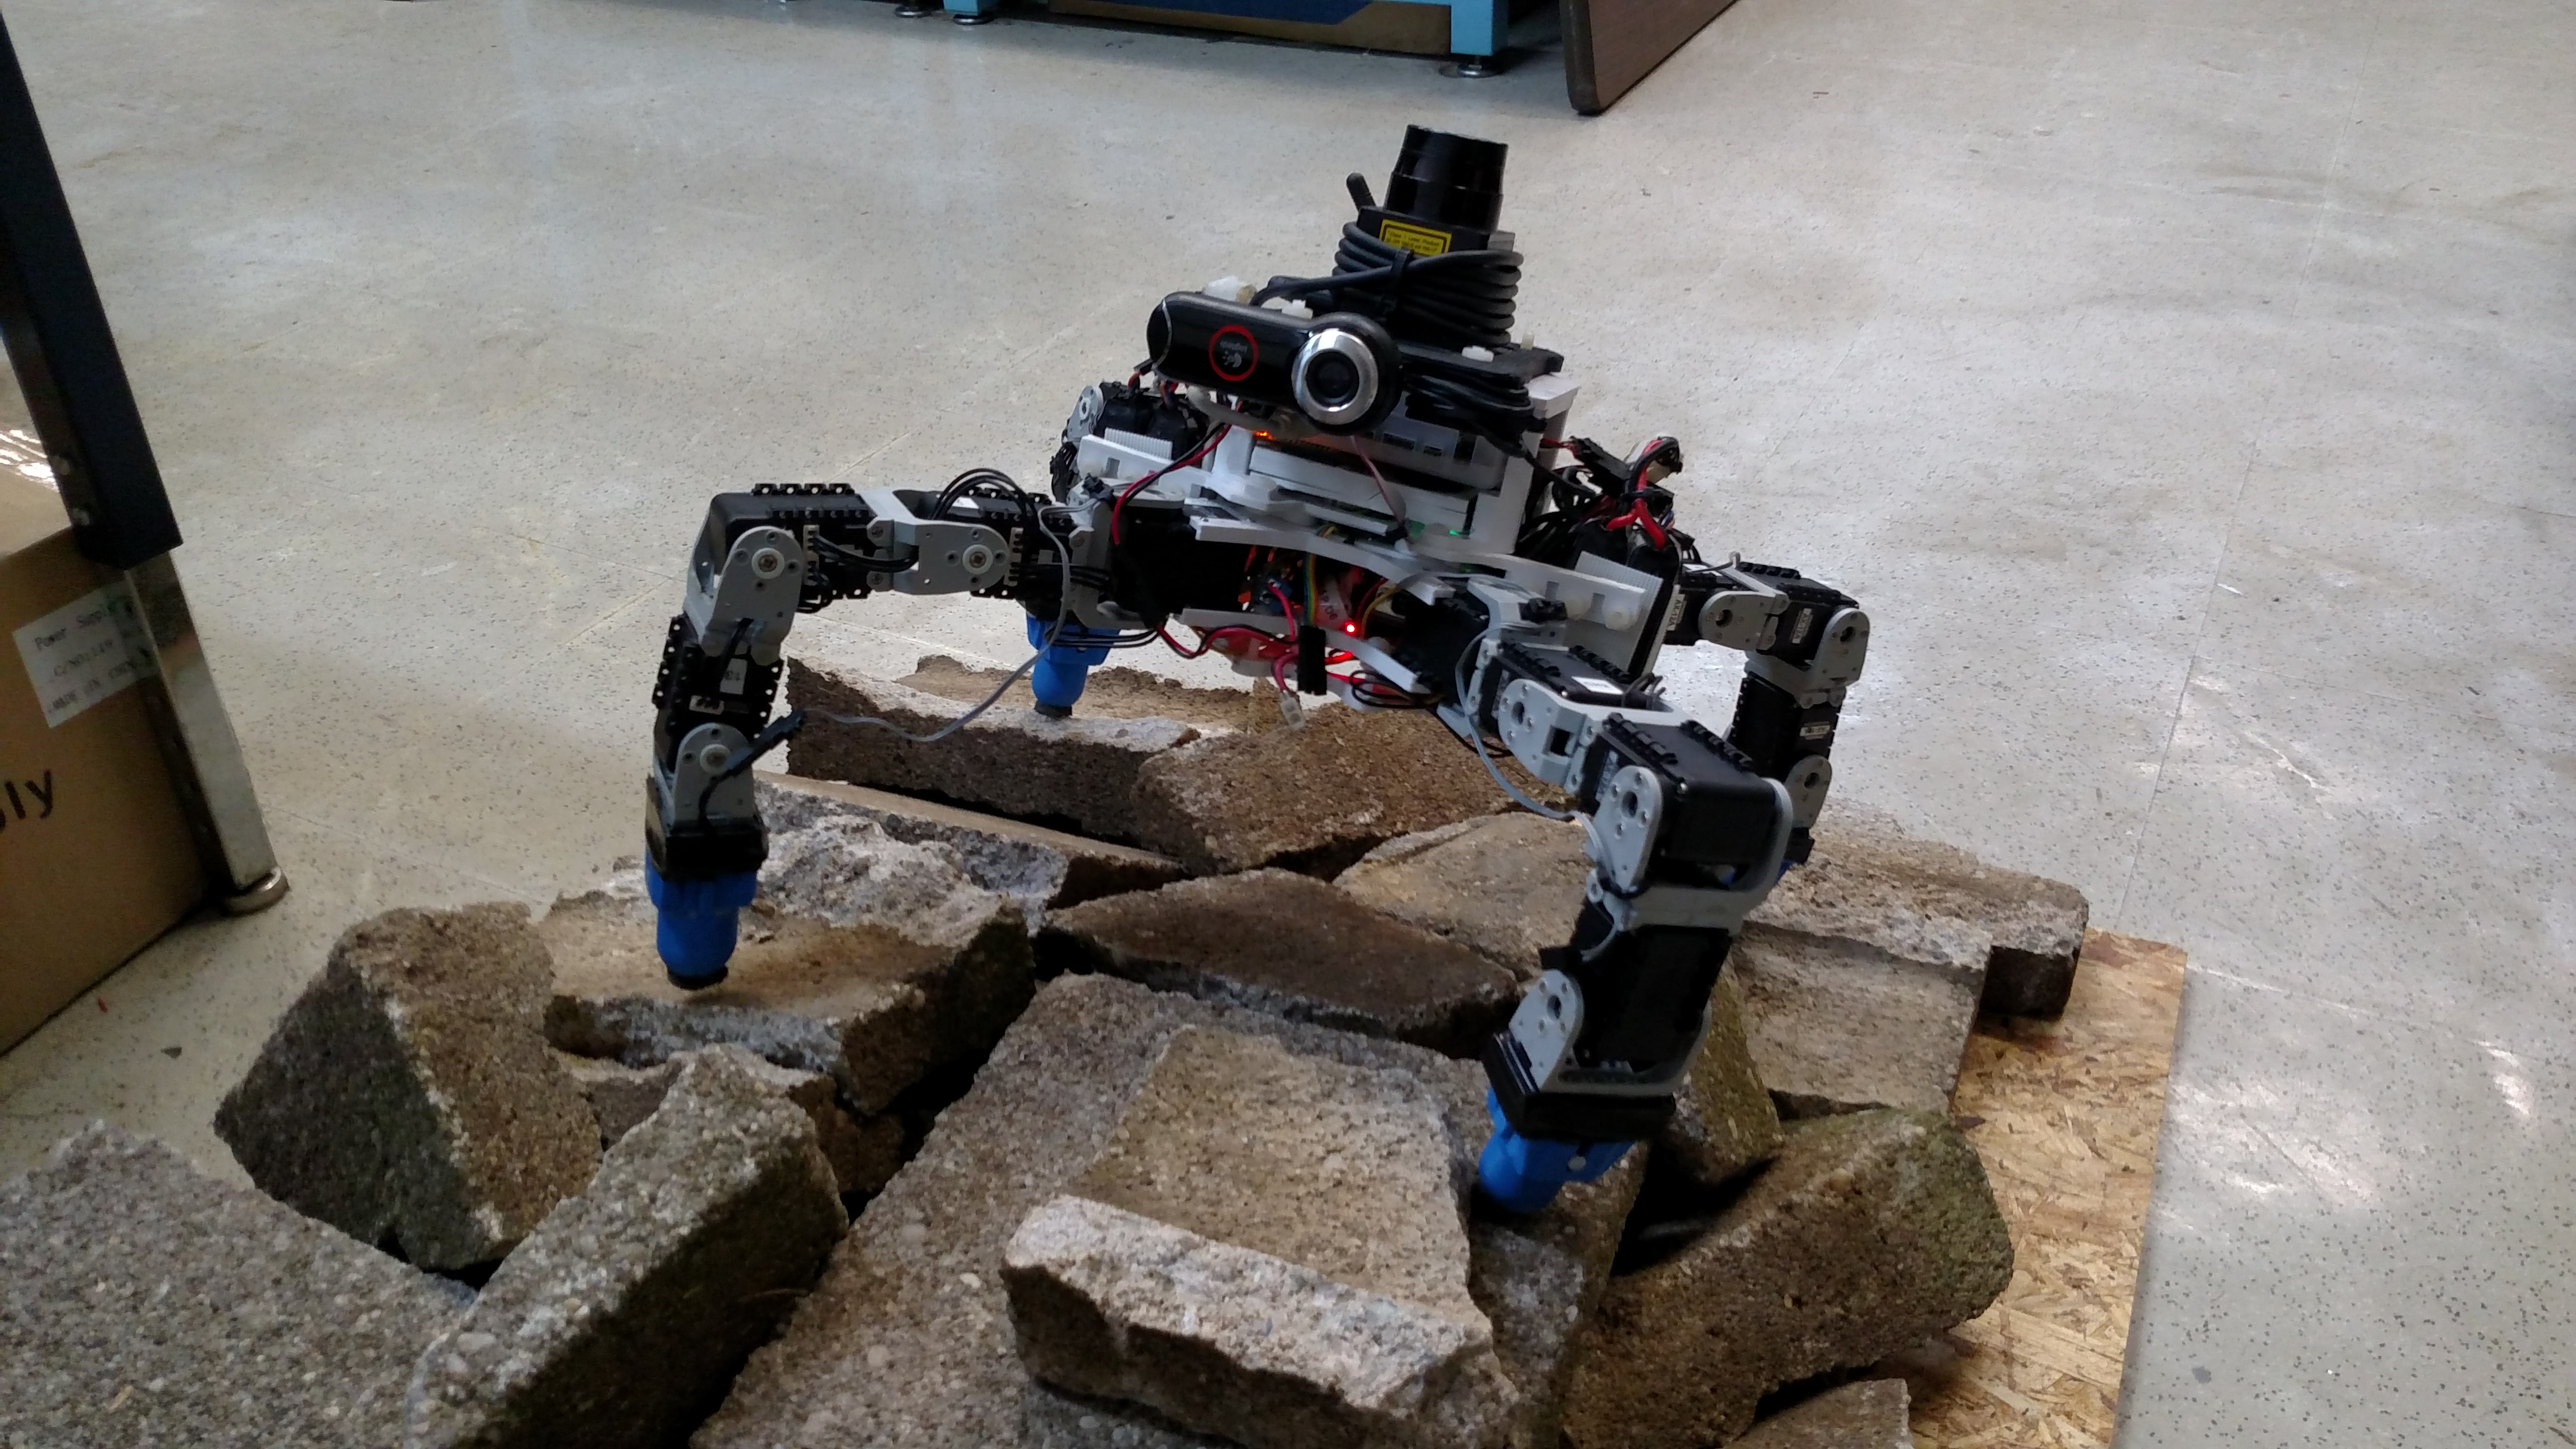
\includegraphics[width=\textwidth]{on_the_rocks2.jpg}}
		\caption{The BlueFoot Quadruped Robot}
		\label{fig::bluefoot_glamour}
	\end{figure}
		The design of legged robots and associated methods of locomotion control has been an area of interest spanning the past several decades, as shown by \cite{McGhee1965,Hodgins1991,Altendorfer2001,Kolter2008,Wieber2015}. Quadruped robotic systems have gained popularity in studies pertaining to variable terrain navigation and full-body stability adaptation. Well known examples of this from the past 15 years are the Tekken \cite{Fukuoka2003}, Kolt \cite{Estremera2006}, BigDog \cite{BigDog2008}, and HyQ \cite{Semini2010_PHD} quadrupeds. Many of these systems have been implemented on a larger scale so that they can carry substantial payloads while maintaining adequate system bandwidth for fast gaits and robustness to rough terrains. Few, however, have been implemented on the scale of a hobby-robot platform while still maintaining an aptitude for rough terrain navigation and comparable sensory prowess.

		The BlueFoot quadruped is a self-contained, fully-actuated platform with the dexterity to perform stabilization and repositioning maneuvers on variable terrains along the same lines as the LittleDog platform \cite{Rebula2007}. Namely, BlueFoot has been designed with 16 actuated degrees of freedom to allow for the execution of a wide range of body and leg articulations. Moreover, BlueFoot's range of articulation allows it to take on a large range of poses during motion. This level of dexterity grants the BlueFoot platform the several notable abilities. For one, it can overcome raised terrain, allowing it to traverse uneven terrain. Additionally, BlueFoot can articulate (\IE pitch and yaw) its on-board vision sensors array, which is attached to its main trunk, by reposing its body through using aggregate leg motion controls. BlueFoot also includes a sizable array of other on-board sensors for feedback and control, including joint position, velocity and loading sensors; an inertial measurement unit (IMU); and foot-contact sensors. Using the computational, sensory and motor capacities at hand, BlueFoot has the ability to utilize similar control mechanisms to those implemented on larger quadruped systems. 

		The BlueFoot platform inherently demands a variety of control routines to achieve locomotion and system stability, making this robot an ample platform for studies related to gait design and motion planning. In particular, BlueFoot's controller considers the systems kinematic model; and involves open-loop gait design and stabilization for the purpose of achieving dynamic locomotion control. In particular, BlueFoot is gaited via a central pattern generator (CPG) based gaiting technique which is augmented with a foothold controller along the same lines as \cite{Ajallooeian2013} and \cite{Rutishauser2008}. Additionally, active platform stabilization is performed via a zero-moment point (ZMP) based body placement controller which stabilizes the system during arbitrary gaiting sequences. The controllers presented here make use of virtual-forces to drive system reference commands and make significant use of the system's forward kinematic model for the purpose estimating the positions of the robot's joints and feet. Finally, outer-loop control routines are implemented to supply commands and corrections used in system navigation control. Among these controllers are a potential fields navigation controller which incorporates image features as target-points to track; and 3D point-cloud processing routines for surface reconstruction and foot-hold planning.

		\section{Central Pattern Generators for Gait Control}

		As previously mentioned, BlueFoot's core gaiting routine relies on the utilization of artificial CPG's, which are inspired from biological neural networks which generate rhythmic motions \cite{Ijspeert2008}. \cite{Arena2000} describes CPGs as a form of self-organizing cellular neural network, and also explains the a the role of limited feedback in CPG's. Infact, a key feature of these networks is that they can act without explicit feedback inputs, or even without directions from a higher-level command unit, such as a brain. Instead, signals emanating from independent motor units and feedback gathered from sensory neurons are utilized to trigger or inhibit a sequence of successive, self-coordinated motor operations. The activation sequences performed by a series of neural unit combine in phase-locked loops create cyclic motion patterns. In robotics, biological CPG's have inspired an artificial counterpart in which neural units are represented by multi-state unit-oscillator. The dynamics of these unit oscillators are coupled with other oscillators within the artificial CPG network. Typically, the CPG network is implemented on a controller, which numerically integrates the dynamics each neural oscillators. The output states of each unit-oscillator are used to drive selected degrees of freedom of a robot system through actuator reference-command signals. Oscillator outputs could also be used for planning periodic motions in the robot's task space, which are then translated into the joint-space via an inverse kinematics mapping, as is done in BlueFoot's gait control routine. The motions produced using the dynamical outputs of each unit-oscillator are usually coordinated through the careful tuning of oscillator coupling, which incurs particular phase offsets between the individual limit-cycles. This stable coordination between oscillators is what allows the CPG to be applied to the performance of a higher-level motor task, such as walking.

		Studies dealing specifically the application of CPG's to multi-legged robot gaiting (specifically quadruped, hexapods and octopodal robots) have been carried out by \cite{Arena2001,Klaassen2002,Arena2004,Inagaki2003,Inagaki2006,Billard2000,Brambilla2006,Buchli2006,Tsujita2001,Tsujita2004}.  In particular, \cite{Ijspeert2008} states that the attractiveness of CPG's in the control of legged robot locomotion lies in a resulting ability to decouple robot motor control, \IE walking, from higher-level planning. Additionally, CPG's offer an effective way for smoothly switching between gaiting patterns, \EG walking, trotting, or pacing, by simply modifying only a few control parameters. As a result, the use of CPG's greatly reduces the dimensionality of the gaiting control problem by generating coordinated motions which can be modified to yield different overall motion patterns without explicit modification of each degree of freedom employed in gait execution.

		An important aspect of the CPG-based gait design applied to the BlueFoot platform is the incorporation of feedback mechanisms which modify the aforementioned CPG parameters. The use of feedback to modify the CPG network for the purpose of improving gaiting stability was guided, in part, by the work of \cite{Fukuoka2003,Endo2004}. Namely, BlueFoot's CPG based gait generation incorporates inertial feedback signals into its CPG mechanism by using them to modify oscillator amplitudes and modulate unit-oscillator frequencies. Additionally, instead of using a CPG to control the outputs of individual quadruped joints, CPG outputs are mapped to stepping trajectories and foot-motion execution patterns. This approach yields a gaiting technique which combines the conveniences of CPG-based gaiting with the heightened control precision of explicit foot-step planning in the robot task-space. Moreover, foot-placement is explicitly prescribed via a separate planning mechanism which decoupled from the CPG gait controller. This method allows a CPG-based motion generation method to be applied gaiting over varying terrains.

		Because CPG-based gaits are inherently open-loop motion control routines, a combination of axillary mechanisms must be used in concert with the base CPG gait controller in order to ensure system stability during gaiting. The incorporation of feedback signals to modified CPG parameters aids in achieving this to some degree, but is usually insufficient for stable walking over largely uneven terrains. 
		
		Additionally this method would require very careful parametric tuning to work robustly under a larger variety of terrain conditions. Thus, other means of stabilization have been incorporated into BlueFoot's gaiting routine to aid in stability. In particular, BlueFoot's core stabilization routines make use of a concept formally named \emph{artificial synergy synthesis} in which gaiting is carried out independently of a stabilization control. Namely, body stabilization is performed by a restricted set of the robot's degrees of freedom while gaiting is carried out independently by the remaining \cite{Vuko1972,Yamaguchi1993}. In an original implementation of this technique, adaptations to trunk motion are utilized to stabilize the overall motion of the robot utilizing a ZMP-based approach, as is done here, while gaiting is controlled by a fixed-motion routine. Here, body and foot-placement are both controlled dynamically, but still independently. The outputs of each controller, which specify body and foot placement in the robot task space, respectively, are combined using the robot's inverse kinematics solution, which generates a final set of joint references.

		\section{Zero Moment Point Body Placement Control}

		The zero-moment point (ZMP), which is equivalent to the center of pressure (CoP), is formally defined as the point on the ground beneath a walking system at which the net moment acting upon the trunk (referred to as the tipping moment) is zero \cite{Sardain2004}. The concept of ZMP and its application to legged robotics was originally introduced by \cite{Vuko1972} and expanded upon in \cite{Goswami1999}, both of which describe ZMP theory towards use in the control of biped robots.

		Formally, the ZMP, $p_{ZMP}$, can be defined using a formulation for the CoP wherein the moments about $\tau_{x}$ and $\tau_{y}$, the tipping-moments applied to the robot's body in the world frame, are equal to zero. The solution for $p_{ZMP}\in\Re^{3}$, with respect to a set of $N$ foot contact points $p_{i,e}\in\Re^{3}$ and $N$ associated applied foot-contact forces $f_{i,e}\in\Re^{3}$, arises as a bounded set of solutions to the equation
			\begin{equation}
				\sum^{N}_{i=1}\wrap{p_{i,e}-p_{ZMP}}\times f_{i,e} 
				= 
				\left[
					\begin{array}{c}
						\tau_{x}	\\
						\tau_{y}	\\
						\tau_{z}
					\end{array}
				\right]
				=
				\left[
					\begin{array}{c}
						0			\\
						0			\\
						*
					\end{array}
				\right]
			\end{equation}
		where $z$-coordinate of $p_{ZMP}$, $\zcomp{p_{ZMP}}$, is strictly zero, as shown in \cite{Wieber2015}. This expression is derived from an inspection of the dynamics which govern the total angular momentum, $\dot{L}$, about the legged system's center of gravity (COG), $p_{COG}$:
			\begin{equation}
				\dot{L} = \sum_{i=1}^{N} p_{i,e}\times f_{i,e} - m_{T} p_{COG} \times \wrap{ \ddot{p}_{COG} + \vec{g} }
			\end{equation}
		where $m_{T}$ is the total mass of the legged system and $\vec{g}$ is the standard gravity vector. Assuming that all foot-contacts exist on a flat plane, \IE $\zcomp{p_{i,e}}=0\SSep \forall i=[1,...,N]$, and all contact force, $f_{i,e}$ are pointing upward, the $p_{ZMP}$ of the system can be written as
			\begin{equation}
				p_{ZMP} 
				= 
				\frac{ \sum_{i=1}^{N} \wrap{ p_{i,e} \times f_{i,e} } }{ \sbrack{\sum_{i=1}^{N} f_{i,e}}_{z} }
				= 
				\frac{ 	p_{COG} \times \wrap{ \ddot{p}_{COG} + \vec{g} } + \dot{L}m_{T}^{-1} }{ \zcomp{ \ddot{p}_{COG} + \vec{g} }}
				\in \emph{C}_{ZMP} 
			\end{equation}
		where
			\begin{equation}
				\emph{C}_{ZMP} = \convhull{p_{1,e},p_{2,e}...,p_{N,e}}
			\end{equation}
		with $\text{conv}(*)$ defining a convex hull from the  input points, $(*)$, and is used to represent the solution space of $p_{ZMP}$. Moreover, $\emph{C}_{ZMP}$ places a bound on the angular momentum $\dot{L}$ which results from contact variations presented through $p_{i,e}$ and $f_{i,e}$. Setting $\dot{L}=0$, we defined a condition for zero tipping. For BlueFoot's ZMP controller formulation, it is also assumed that the acceleration of the COG is sufficiently small, \IE $\ddot{p}_{COG}\approx0$ which yields the following, intuitive stability condition:
			\begin{equation}
				\norm{p_{ZMP} - p_{COG}} < \epsilon
			\end{equation}
		where $\epsilon\ll1$ is a small bounding constant. Thus, the general idea of this ZMP-based controller is to compute an approximate ZMP location and place the center of the robot's trunk (described by the translation $p_{b}$) such that the platform's COG approaches its associated ZMP for some arbitrary kinematic configuration, thus minimizing $\norm{\dot{L}}$ so as to avoid tipping.


		\section{Trunk stabilization}

		In addition to the aforementioned task-space controllers, a learning controller, which features the use of a NARX neural network is used to aid trunk stability has been studied. In essence, this controller learns to approximate disturbance dynamics during periodic gait routines and corrects trunk orientation by administering adaptations to joint position controls. The goal of such control routine is to achieve a level trunk during locomotion.
			
		A NARX-NN architecture is used in this controller because of  its known effectiveness in approximating nonlinear difference systems and making multivariate time-series predictions \cite{Tsungnan1996,ChenBillings1990,Hihi1996,Billings2013}. Moreover, the NARX-NNs is a natural fit for a problem of this nature where the dynamics being considered are both periodic and of a high enough complexity where a nonlinear approximation method is warranted. The parallel NARX-NN model, shown in Figure \ref{fig::narx_net}, is comprised of a feed-forward neural network whose input layer accepts a series of time-delayed system state values and network-output histories. The NARX-NN is trained to predict system states in the next time-instant from these inputs. Conveniently, NARX-NN training can be performed using standard BP because recurrence occurs between network inputs and outputs, and not within the hidden layers \cite{Nelles2001}.

		The NARX-NN is trained to capture the effects of forces and moments and dynamical couplings that act on the trunk so that an appropriate torque input to the joints is computed to reduce such effects on trunk orientation while performing the gate. This is achieved by considering the inverse dynamics corresponding to joint motion.

		Disturbances imparted upon the trunk during gaiting manifest in the term $\Phi$, largely as a result of variations in $f_{ext}$ and associated effects due to dynamical coupling. Because of this, the NARX-NN will learn an estimate for $\Phi$, denoted $\hat{\Phi}$. The network is trained on-line using the standard incremental back-propagation (BP) algorithm with an adapted learning rate, $\gamma^{lr}$ and momentum term, $\mu$ \cite{Rumelhart1988,Rumelhart1995}. This error BP algorithm is a gradient-descent based method used to train a feed-forward neural network with $n$-layers and layer-connection matrices $\setwrap{W^{1},W^{2},...,W^{n-1}} \in \emph{W}$. The BP algorithm, as used in this control approach, is summarized in matrix-vector form in (adapted from \cite{Rojas1996ch7}) as follows: 

		\begin{equation}
			\Delta W^{i} =
				-\gamma^{lr} \wrap{ \frac{ \partial o^{i} }{\partial {W^{i} } }  o^{i-1} }^{T}  + \mu \Delta W^{i} = 
				-\gamma^{lr} \delta^{i} \wrap{o^{i-1}}^{T}  + \mu \Delta W^{i}
			\label{eq::bp_weight_update}
		\end{equation} 
		%
		where
		%
		\begin{equation*}
			\delta^{i} = \wrap{ \nabla_{y} \sigma^{i}\wrap{y^{i}} } e^{i}
			\label{eq::bp_error}
		\end{equation*}
		\begin{equation*}
			y^{i} = W^{i} o^{i-1}
			\label{eq::bp_error}
		\end{equation*}
		\begin{equation*}
			e^{i} =  \wrap{ W^{i} }^{T} \delta^{i+1} \hspace{2mm} \forall \hspace{2mm} i\neq n,
		\end{equation*}
%%
		$\gamma^{lr} \in [0,1]$, the learning and  $\mu \in [0,1]$, the learning momentum; $W^{i} \in \Re^{N_{O}^{i}\times N_{I}^{i}}$, which represents the weighting matrix between the \Ith layer (of size $N_{I}^{i}$ nodes) and $(i+1)^{th}$ layer (of size $N_{O}^{i}=N_{I}^{i-1}$); $\Delta W^{i}$, which represents the corresponding weight update to $W^{i}$; and $e^{i}$ is the output error for each \Ith layer. For the output ($n^{th}$) layer, $e^{n}$ is equal to the difference between the network output and the network output target, which will be defined later. For all other layers, $e^{i}$ represents a \emph{back-propagated} error. from the $(i+1)^{th}$ layer.

%%
		$\sigma^{i}(y^{i})$ is a layer-wise activation function which outputs a vector of scalar activation outputs, $\sigma_{j}^{i}(y_{j}^{i}) $ for each \Jth, weighted input, $y_{j}^{i}$, defined as follows:
		\begin{equation*}
			\setwrap{ \sigma^{i}(y^{i}) = \sbrack{ \sigma_{1}^{i}(y_{1}^{i}),...,\sigma_{N_{I}^{i}}^{i}(y_{N_{I}^{i}}^{i}) }^{T} \hspace{2mm} : \hspace{2mm} \Re^{N_{I}^{i}} \rightarrow \Re^{N_{I}^{i}}}
		\end{equation*}
		For the trunk-leveling controller being described, a symmetric sigmoid activation function is used, making each $\sigma_{j}^{i}(y_{j}^{i}) \equiv \tanh(y_{j}^{i}) \in [-1,1]$. Hence the gradient $\nabla_{y} \sigma^{i}(y^{i})$ is defined as follows: 
		\newcommand{\acti}[1]{\sigma^{#1}_{1}(y^{i})}
		\begin{equation}
			\nabla_{y} \sigma^{i}(y^{i})  =
			\left[
			\begin{array}{cccc}
				\acti{1}	&	0		&	\ldots 		&	0 			\\	
				0			&	\acti{2}&	0			& 	\vdots 		\\
				\vdots 		&	0		& 	\ddots 		& 	0			\\
					0			&	\ldots	&	0			& 	\acti{N_{I}^{i}}
			\end{array}
			\right]
			\wrap{\vec{1}_{N_{I}^{i}\times1} - \sigma^{i}\wrap{y^{i} } }
			\label{eq::bp_sigmoid_deriv}
		\end{equation} 
		given the derivative properties of the $\tanh\wrap{*}$ function.
		
		The success of this learning mechanism, as it applies to the presented controller, is predicated on the periodicity of the system dynamics during gaiting. Like any BP-trained neural network, repetition of similar input and output sets is paramount for successful network training and, by extension, prediction accuracy. It is assumed that this specification can be met given the inherently cyclic nature of the dynamics being estimated during gaited locomotion. 
		%%%
		%%%
			\begin{figure}[t!]
				\centering
				\fbox{\includegraphics[width=1.0\textwidth]{narx_network_diagram.png}}
				\caption{Parallel NARX-network model with a linear output layer.}
				\label{fig::narx_net}
			\end{figure}
		%%%
		%%%

		\section{Navigation and 3D Reconstruction}

		One method that has been selected for navigating the BlueFoot platform over flatland is a potential-fields control approach, described in \cite{Hogan1984} for the purpose of controlling robotic manipulators, and analyzed in-depth in \cite{Koren1991}. In particular \cite{Koren1991} presents shortcomings of this approach. Nonetheless, a potential fields navigation methods offers a reflatively simple and intuitive approach to robot navigation and fits well into mobile robotic tasks which involve ``wandering'' type navigation over flat regions, in which the robot has yet to aquire any knowledge of surrounding obstacles. In this thesis, a potential fields navigation approach is used to navigate BlueFoot in unknown regions, and is coupled with camera-based feature tracking to guide the robot towards potential areas of interest within an unknown, immediate space.

		The potential fields approach is used in mobile robot navigation by moving the robot according to a guiding virtual force-vector, $F_{nav}$ \cite{Koren1991,ArambulaCosio2004}. This vector is comprised of a sum of virtual repuslive forces, $F^{-}$ (typically generated range-sensor data), and virtual attractive forces, $F^{+}$, which pull the robot towards known goals. Thus $F_{nav}$ formally defined as:
		%%%
		\begin{equation}
			F_{nav} = F^{+} + F^{-}
			\label{eq::sumofforces}
		\end{equation}

		The general form for the force components $F^{+}$ and $F^{-}$ (represented as $F_{c}$) is as follows:
		%%%
		\begin{eqnarray}
			d_{k} 	&=& p_{POI,k} - p_{robot} \nonumber\\
			F_{c}	&=& \alpha_{F}\sum_{k}\wrap{ f(\norm{d_{k}})\frac{d_{k}}{\norm{d_{k}}} }
			\label{eq::sumofforces}
		\end{eqnarray}	
		where $p_{poi}$ and $p_{robot}$ are position of each \Kth point-of-interest (POI) and the position of the robot platform; $f(*)$ is a potential function which returns a scalar ``energy" factor with respect to a scalar distance argument $(*)$; and $\alpha_{F}$ is a scaling parameter which is positive for when POIs represent goals and negative when POIs represent obstacles to avoid. The potential function and force-scaling factors are designable for particular applications. For BlueFoot's navigation scheme, attractive and repulsive forces are generated using a single, consolidated forcing function which is used to guide through an environment even when a goal is not specified before hand. 

		The aforementioned potential field navigation method is used, primarily, to handle BlueFoot's flatland navigation. Navigation over rough terrain requires a number of other considerations about the terrain of the enviroment itself, as opposed to simple POIs which can be resolved by observing the enviroment around the robot in 2D. Thus, surface reconstruction plays a large roll in the process of navigation over irregular terrain. This thesis will present two methods of surface reconstruction, which will serve as prelimaries for rough-terrain navigation and planning in futurer work with the BlueFoot platform.

		\section{Overview of Thesis}

		This thesis will first detail the major hardware components; design considerations; and construction of the BlueFoot platform. Next, the software and processing architecture used to control the BlueFoot platform will be described. Thereafter, the kinematic and dynamical model of the BlueFoot system will be described, followed by control routines which are presently implemented to gait, stabilize, and navigate the BlueFoot platform. The final section of this thesis will contain concluding statement about the system design and control, including remarks about possible future directions of study related to the BlueFoot platform and legged robotics as a whole.

	\include{ch2_hardware}
	\label{ch::software}
%%%%%%%%%%%%%%%%%%%%%%%%%%%%%%%%%%%%%%%%%%%%%%%%%%%%%%%%%%%%%%%%%%%%%%%%%%%%%%%%%%
%%% Software
%%%
%%% Section 1 : Software Architecture
%%% 
%%% Section 2 : Ground Station
%%%
%%% Section 3 : Simulator
%%%
%%%%%%%%%%%%%%%%%%%%%%%%%%%%%%%%%%%%%%%%%%%%%%%%%%%%%%%%%%%%%%%%%%%%%%%%%%%%%%%%%%
\chapter{Software}
	
	\section{System Software Architecture}
	
	BlueFoot is controlled using a multi-processor software architecture which incorporates several independent control-software cores. Each software core handles specific subsets of operations essential to the macro-system. This distributed system architecture allows independent tasks (such as actuator command/feedback handling, battery monitoring, etc.) to be decoupled from more computationally heavy tasks by offloading them to physically separate computing modules. Therefore, each control unit handles an assigned task set in an independent control loop which contribute updates to the overall macro-system in an asynchronous fashion. System control tasks are divided into four main categories, which can be summarized as follows:
		\begin{itemize}
			\item{
			\emph{Low-Level Control} : 
				power monitoring/switching, 
				actuator command handling, 
				communications routing,
				sensor data acquisition,
				script parsing and evaluation
			}
			\item{
			\emph{Motion/Motor Control} : 
				gait planning, 
				gait adaptation, 
				trunk pose adaptation
			}
			\item{
			\emph{High-Level Control} : 
				vision sensor handling,
				perception, 
				motion planning, 
				surface reconstruction, 
				navigation, 
				localization
			}
			\item{
			\emph{Human-Operator Control} : 
				joystick/keyboard commands,
				scripting commands
			}
		\end{itemize}
	As previously mentioned in Chapter \ref{ch::hardware_and_design}, low-level and motor/motion control tasks are handled, exclusively, by the Lower Brain (LB), which is comprised of a software collective spanning over the RM48 and TM4C processors on-board the AutoPilot. High-level control tasks are handled by the Upper Brain (UB), which is the software-core which runs on the ODROID-XU module. Lastly, a human operator can interface with the system wirelessly from a personal computer running ground-station software. This ground station software which communicates directly with the TM4C processor. The ground-station also interfaces with the UB over an SSH connection. This secondary wireless connection is used, mainly, for on-board data-logging configurations.

	Since this software architecture is distributed over several separate computational units, an integral part of this control architecture is an efficient, reconfigurable interprocessor communication protocol. Namely, BlueFoot utilizes data packets transfered over serial lines to update system states between processors. These data packets are formatted using a binary-XML protocol, called EXI. This protocol facilitates a highly customizable packeting structure for asynchronous inter-module communication and utilizes robust packet-error checking routines. This sections will detail the specifics of BlueFoot's interprocessor communication protocol, namely the composition of packets transferred between processor. 

	This section will also detail the specific software-level tasks handled by each of BlueFoot's processor; the speed at which each core software element is run (update frequency); and what data must be communicated between software elements for operation. Additionally, this section will describe the ground-station software and corresponding user-interface used to control the BlueFoot Quadruped and administer high-level commands.
	
	\subsection{System Task Allocation}

		\begin{figure}[h!]
			\centering
			\fbox{\includegraphics[width=\textwidth]{process_diagram.png}}
			\caption{BlueFoot's main processes and their relationships.}
			\label{fig::process_diagram}
		\end{figure}

		Figure \ref{fig::process_diagram} depicts how core software and associated control elements are related within the BlueFoot software macro-system. This section will detail a general description of the tasks carried out by each major software module implemented on the BlueFoot quadruped.

			\subsubsection{TM4C (Lower Brain)}

			As previously mentioned, the TM4C processor on-board the AutoPilot module is responsible for \emph{Low-Level} tasks and can be viewed a safety/communications routing co-processor within the overall system. Within its main program loop, the TM4C polls the system's main battery voltage via ADC interface routines; handles transmit and receive (packet decoding) routines between the ground-station and the RM48 system nodes; and handles command dispatching and feedback polling with the system's 16 servo actuators. The TM4C is directly interfaced with two dual-channel power switching IC's and is used to control power supply to each leg by toggling general purpose IO pins in software. The state of these pins is administered as part of a periodic packet command/update packet sent from the ground-station. Since the TM4C has this control over the system's actuators (which consume most of the system's power) and battery monitoring capabilities, it runs a safety routine which is responsible for halting motor activity and/or cutting system power on low-battery or power-fault conditions, as well as during unexpected breaks in communication with the ground-station.

			As previously mentioned, the TM4C handles communication routing between system processing modules; as well as with controllers on-board each smart-servo. Administering servo commands and collection servo feedback it the TM4C's highest priority task. This process, which involves both commanding and requesting feedback from each servo, is relatively expensive  and limits the TM4C's loop frequency to roughly 50 Hz. Thus, it is particularly important that this task is offloaded to this processor, as its other safety and communication-related tasks are much less expensive, by comparison, and allow the servo actuators to be updated quickly as possible without encumbering other system control operations.


			\subsubsection{RM48 (Lower Brain)}

			The RM48 is responsible for several \emph{Low-Level} tasks, including IMU polling and handling communication with the TM4C and ODROID-XU. Each collected IMU sample is passed along to an extended Kalman Filter routine, which generates a trunk orientation estimate, $\hat{\theta}_{b}$ in the world frame, $O_{0}$. 

			The RM48's primary function is to carry out motion control and gait-planning tasks. To achieve this, the RM48 handles a state machine which switches between planned motion execution and trajectory control; and gait control via a Central Pattern Generator (CPG) based gaiting controller, which will be discussed in more detail in Chapter \ref{ch::gait_control}. Additional functions for body and posture (position and orientation) control, including trunk leveling procedures, and gait-stabilization are run in tandem with the aforementioned gait-control task.

			Motion and gait controls, which are performed in the robot task-space, are converted into joint-space reference angles, $q^{r}$, via an inverse kinematics (IK) routine. The IK routine is exectued at all times when the legs are engaged for the purpose of issuing servo position commands, given desited task-space configurations for body and feet positions, which will be more formally defined in Chapter \ref{ch::system_modeling}. The RM48 also maintains BlueFoot's forward kinematic model (specifically, foot position relative to the trunk), which relies on an EKF-generated trunk orientation estimate, $\hat{\theta}_{b}$, and joint position feedback, $q$. BlueFoot's inverse and forward kinematics models will be detailed in Chapter \ref{ch::system_modeling}. The RM48 runs its full control loop at approximatively 100 Hz (twice the speed of the TM4C control loop) to facilitate higher integration stability when updating gait related controller dynamics, dynamic motion controls, task-space reference trajectories.

			Lastly, the RM48 handles an on-board scripting engine (based on the MIT Squirrel Scripting), which interprets lexical commands. This scripting engine is capable of handling a large number of high-level commands [http://squirrel-lang.org/] and is complex enough to handle function and class definitions in real time. The scripting engine currently being used to evaluate BlueFoot's core user command set, ranging from simple state toggling and parameter modification, to the prescription of user-specified way-points for navigation, among other high-level command itams. Scripting commands are passed from the ground station (via terminal) and routed through the TM4C to the RM48, where they are finally evaluated.


			\subsubsection{ODROID-XU (Upper Brain)}

			The ODROID-XU runs software upon a Debian (Linux) operating system distribution ``Jessie." The use of an Linux operating system extends itself to a number of programmatic conveniences, such as to ability to run several tasks in parallel threads. Inbuilt USB drivers are used in functions which are used to acquire data from USB-interfaced vision sensors. Namely, the ORDOID runs sensor handling elements used for acquiring and buffering camera images and controlling camera frame-rate control; as well as LIDAR scan frames. The ORIOID uses these sensor inputs, in conjunction with orientation estimates and inertial data passed from the RM48 to perform several navigation-related tasks (\EG potential fields, mapping, localization, terrain-reconstruction). These tasks will be described in more detail in Chapter \ref{ch::navigation}.

			The ODROID utilizes 2D-LIDAR scans (frames) and trunk-pose estimates to form organized 3D point clouds. These point-clouds are further processed to reconstruct 3D terrain surfaces and height-maps, which are then used for step-planning. LIDAR frames are utilized in potential fields-based navigation tasks. These navigation modes also incorporate camera data for the purpose of goal-targeting (where the goal is typically an object of particular shape or color). Image processing and image feature detection is run as a separate process on the ODROID, which is incorporated with the aforementioned processed sensor data to produce a set of forward and turning velocity commands, $v_{r}$ and $\omega^{r}$, respectively; as well as foot-hold positions generated from step-planning algorithms. In particular, the open-source libraries OpenCV (Open Computer Vision Library), OpenPCL (Open Point-Cloud Library), and Boost are heavily used in the software developed to carry out the aforementioned tasks. Software written for this platform was generated using a mixture of C++ and Python.

			As previously mentioned, the ODROID can handle a limited set user-command on its own, which are administered directly to the ODROID from an SSH terminal on the ground-station computer. These commands include core-program start-ups and data-logging configurators. Essentially, the ODROID's software core is designed as a completely independent software module which replaces the roll a human director, as it handles the bulk of the systems high-level planning and navigation tasks. Moreover, if the ODROID is removed from the BlueFoot system, the system can still be operated via remote-control heading commands provided from human operator (\IE ground-station joystick control).
		
		\subsection{Inter-processor Communication}

			\begin{figure}[h!]
				\centering
				\fbox{\includegraphics[width=\textwidth]{comm_flow.png}}
				\caption{Communication flow between processors on the BlueFoot Platform.}
				\label{fig::comm_flow}
			\end{figure}

			This section will detail the contents of the data packets transfered between processors, which is summarized in Figure \ref{fig::comm_flow}. System directives, generated by a human operator who interacts with the robot via a graphical user interface and/or joystick controllers, are generated from a ground-station computer. Packets (without padding) sent from the ground station to the BlueFoot robot (TM4C) are composed as shown in Table \ref{tab::gs_to_tm4c_packet}:
			\begin{table}[h!]
				\centering
				\begin{tabularx}{\textwidth}{|C{0.2}|C{0.2}|C{0.2}|C{0.2}|C{0.2}|} 	
					\hline
					\emph{32-bits} 	& \emph{8-bits} 		& \emph{8-bits} 	&\emph{16-bits} 	& \emph{16-bits} 	\\\hline
					HEADER 		& Master-Tog.		& Power-Tog.	& Unused		& Network Info 	\\\hline
					\emph{Variable} 	& 		 		& 			&			& 			\\\hline
					Scripts 		& 				& 			& 			&			\\\hline
				\end{tabularx} 
				\caption{Structure of the packets sent from Ground-Station to TM4C.}
				\label{tab::gs_to_tm4c_packet}
			\end{table}
			
			Every packet issued using the EXI protocol has a 4-byte (32-bit) header. As part of the internal system protocol, every packet sent between system nodes contains a ``Master Status Vector", which is comprised of a fixed length, 7-byte sequence of essential system information/control items. The ``Master Toggles" section (first 8-bits after header) enumerate major systems states, including \emph{On-line, Standby, Off-line} and \emph{Suspended} system state designations. The next 8-bits are used to toggle on-board power, namely the power supplied to each leg. The remaining 32-bits are used for specifying battery voltage (8-bits), power-fault states (8-bits), generic binary feedback toggles (8-bits), and system networking information (16-bits). The last section of this packet contains scripting commands, which can be of varying lengths. For example, foward velocity and turning rate commands (gathered form a joy-stick controller) are administered in the form of scripted commands.

			Packets sent from the TM4C to the Ground-station contain status items generated on board the robot, and appear as shown in Table \ref{tab::tm4c_to_gs_packet}:
			\begin{table}[h!]
				\centering
				\begin{tabularx}{\textwidth}{|C{0.2}|C{0.2}|C{0.2}|C{0.2}|C{0.2}|} 	
					\hline
					\emph{32-bits} 	& \emph{8-bits} 		& \emph{8-bits} 	& \emph{8-bits} 	& \emph{16-bits} 	\\\hline
					HEADER 		& Master-Tog.		& Unused		& Foot-Contacts	& Network Info 	\\\hline\hline
					\emph{2048-bits} 	& 				&			&  			& 		 	\\\hline
					Joint Pos. FB		& 				& 			& 			& 			\\\hline
				\end{tabularx} 
				\caption{Structure of the packets sent from the TM4C to the Ground-Station.}
				\label{tab::tm4c_to_gs_packet}
			\end{table}
			The \emph{Joint Pos. FB} (joint position feedback) element is composed of 16 2-byte sequences corresponding to the joint positions of read-back by each actuator. To avoid redundancy, the structure of the packets communicated from the TM4C to the RM48 and vice-versa will not be depicted explicitly. Like all system packets, these packets contain a 7-byte master status vector with only the \emph{Master-Toggle} and \emph{Network Info} fields populated. The TM4C sends the same joint feedback information to the RM48 as it does the Ground Station. For packets sent from the TM4C to the RM48, this field is replaced with corresponding joint-position commands for each of the 16 servo actuators. This field is also 2048 bits in length.

			Packets sent from the RM48 to the ODROID contain additional dynamical-state fields for use in planning on the ODROID. State information is sent in the form a vectors with 32-bit, single precision floating-point elements. This set of information includes trunk a orientation estimation, angular rate, and global position (generated from open-loop command integration), each of which are represented as 3-element vector; and foot-position estimates (four, 3-element vectors.) generated. These packets have a structure which is depicted in Table \ref{tab::rm48_to_odroid}.
%
			\begin{table}[h!]
				\centering
				\begin{tabularx}{\textwidth}{|C{0.2}|C{0.2}|C{0.2}|C{0.2}|C{0.2}|} 	
					\hline
					\emph{32-bits} 	& \emph{8-bits} 		& \emph{8-bits} 	& \emph{8-bits} 	& \emph{16-bits} 	\\\hline
					HEADER 		& Master-Tog.		& Unused		& Foot-Contacts	& Network Info 	\\\hline\hline
					\emph{96-bits} 	& \emph{96-bits}		& \emph{328-bits}	&\emph{328-bits}  	& 		 	\\\hline
					Orientation		& Angular Rate		& Trunk Pos.		& Foot Positions	& 			\\\hline
				\end{tabularx} 
				\caption{Structure of the packets sent from the RM48 to the ODROID.}
				\label{tab::rm48_to_odroid}
			\end{table}
Packets sent form the ODROID to the RM48 contain command items, such as forward velocity, turning rate and trunk-pose commands, as well as foothold-references and corrected global trunk position estimates. These packets are constructed as shown in Table \ref{tab::odroid_to_rm48} :
%
			\begin{table}[h!]
				\centering
				\begin{tabularx}{\textwidth}{|C{0.2}|C{0.2}|C{0.2}|C{0.2}|C{0.2}|} 	
					\hline
					\emph{32-bits} 	& \emph{8-bits} 		& \emph{8-bits} 	& \emph{8-bits} 	& \emph{16-bits} 	\\\hline
					HEADER 		& Master-Tog.		& Unused		& Unused		& Network Info 	\\\hline\hline
					\emph{32-bits} 	& \emph{32-bits}		& \emph{96-bits}	&\emph{328-bits}  	& \emph{96-bits} 	\\\hline
					Velocity		& Turning Rate		& Trunk Pose		& Footholds.	& Trunk Pos.		\\\hline
				\end{tabularx} 
				\caption{Structure of the packets sent from the ODROID to the RM48.}
				\label{tab::odroid_to_rm48}
			\end{table}

	\section{Ground Station}
		
		\begin{figure}[h!]
			\centering
			%\fbox{\includegraphics[width=\textwidth]{comm_flow.png}}
			\caption{The BlueFoot ground-station GUI.}
			\label{fig::comm_flow}
		\end{figure}

	Ground-station software used for controlling the BlueFoot platform was generated in C++ using an open-source graphical user interface design library called \emph{wxWidgets} [Need ref]. \emph{wxWidgets} is used, primarily, for the ground-station's front-end design. Namely, the ground-station code is designed such that that its US design is reconfigurable via an XML-based design specification file. Furthermote, this allows for UI reconfigurations without the need to change internal, back-end processes. In terms of the GUI backend, \emph{wxWidgets} handles general UI signal processing, and allows for easy registration of user callbacks on events such as button presses. Additionally, \emph{wxWidgets} provides an interface for collective joystick inputs, which are interpretted and sent to the BlueFoot as remote-control commands. \emph{Boost}, a C++ utility library, is utilized to provide socket and serial-port IO handling. This library is particularly important for use with the ground-station's wireless radio, which transmits information to the robot from data sent to the radio module over USB.  

	 The ground station is composed of several main UI sections which allow for system master-state, opterating-state and power toggling; administering system commands and script. Basic system state controls are used to periodically populate a fixed-structure, robot-command packet, shown in Table \ref{tab::gs_to_tm4c_packet}. This packet is used to refresh the robot operating state and manually-set navigation commands, and is sent to the platform rate of 25 Hz using the an XBEE radio module. BlueFoot replies to each ground-station update with a packet of internal configurations, as shown in Table \ref{tab::tm4c_to_gs_packet}, which is then used to ensure that system updates and command are being adminstered properly and that the system is live.

	Namely, BlueFoot sends the following particles of system information back to he ground-station: battery voltage levels; power fault coniditons; foot contact feedback; and joint position feedback. This data is used to update several key portions of the UI. Firstly, battery levels are used to update a battery meter, which indicates the current system voltage level. Additionally, a dynamic text box displays the system's power-fault state to the user. Joint position commands are used to update a visualization of the robot in real time. The foot-color of the vizualized BlueFoot robot changes from blue to red to represent foot-contact conditions. Joint positions, foot-contact states and battery levels are time-stamped and automatically logged during each ground-station session for later analysis. 


	\include{ch4_modeling}
	\chapter{Gaiting and Gait-Stability Control}
\label{ch::gait_control}



	\section{Overview}

		Legged robotic systems have long employed motion controllers based on limit cycle oscillators and, more recently, Central Pattern Generators (CPGs)  for the purpose of generating bio-mimetic gaits \cite{Matsuoka1985,Collins1993,Endo2004,Righetti2006,Ijspeert2008,Matos2010,Ajallooeian2013,Park2014,Fukuoka2015}. Since these motion control methods are open-loop motion planners (\IE not inherently formulated to incorporate feedback) they do not perform any active syste stabilization on their own accord. As a result, implementations involving these  locomotion methods often require auxiliary control mechanisms which provide gait stability. Fixed point methods, which include considerations of the system's zero-moment point (ZMP) and center of gravity (COG), are utilized in the design of stable oscillator driven gaits. These methods are summarized in \cite{Wieber2015}. %add ZMP references%

		Developments in CPG-based gait controllers have led to the incorporation of ``reflexive" feedback mechanisms aimed at correcting foot-placement during gaiting on uneven terrain or various surfaces. One such approach involves active compliance to each leg by directly modifying CPG oscillators units through feedback-driven modulations. In \cite{Fukuoka2003} and \cite{Endo2004}, a CPG for each leg is modified by a neural oscillator with one tuning parameter. 

		This chapter will detail a similar, reflex-adaptive CPG gait generation method which utilizes IMU feedback to modify CPG limit-cycle parameters. Additionally, this section will present related motion-control methods implemented on the BlueFoot platform which aid in gait stabilization, including a virtual force-based foot placement planner and a ZMP-based body placement controller; as well as a nuero-control technique used to level BlueFoot's trunk.




	\section{Central Pattern Generator (CPG) Based Gaiting}

		A central pattern generator (CPG), which includes a reflexive mechanism using sensory feedback, is utilized as the core of the robot's gait generation algorithm. CPGs are a form of neural oscillator network which mimic biological mechanisms for repetitive motor tasks \cite{Ijspeert2008}, \cite{Collins1993}. CPGs commonly consist of a network of multi-state unit-oscillators. These unit-oscillators are coupled such that the motion of one oscillator drives or attenuates the motion of other oscillators it is connected to, creating phase-locked limit cycles.

		In this context, the limit-cycles generated with a CPG will be utilized to drive a quadruped  walking gait by mapping oscillator outputs to foot position controls. CPGs are widely used in this way as they provide a compact method for prescribing rhythmic gaits with variable stepping sequences 
		\cite{
			Righetti2006,
	 		Castro2008,
			Li2014
		}. 
		CPG-driven gait controllers are convenient as they allow for continuous transitioning between gaiting patterns through the modification of oscillator coupling. Reflexes are built into the oscillators which use IMU measurements to modulate the CPGs unit oscillators, as will be outlined later in this section.

		The CPG implemented on BlueFoot consists of four modified two-state ($y_{1,i},y_{2,i}$) Hopf Oscillators connected through a coupling matrix $K$.  The oscilator output vector, $y_{2,i}$, parameterize the trajectories of each \Ith foot. The resulting reflexive CPG system is described by
		\begin{eqnarray}
			\dot{y}_{1} &=& A_{1}\wrap{ \Psi_{M} M - \Gamma}{y}_{1} + \Psi_{\omega} W {y}_{2} 			\nonumber\\
			\dot{y}_{2} &=& A_{2}\wrap{ \Psi_{M} M - \Gamma}{y}_{2} - \Psi_{\omega} W {y}_{1} + K {y}_{2}	%\nonumber
			\label{eq::CPGMain}
		\end{eqnarray}
		where $M$ is a diagonal matrix  in $\Real^{4\times4}$ with diagonal elements $m_{i,i}=y_{1,i}^{2}+y_{2,i}^{2} \Sep \forall i = \{1,2,3,4\}$, $\wrap{A_{1},A_{2}, \Psi_{M}, \Psi_{\omega}} \InRe{4\times4}$, $  \{y_{1}, y_{2}\}  \InRe{4\times1}$, and $\Gamma$ and $W$ are diagonal matrices in $\Real^{4\times4}$ which represent nominal oscillator amplitudes and frequencies, respectively.


		\subsection{Reflexive Gait Adaptations}


			Feedback signals are incorporated into the CPG through the frequency modulation matrix $\Psi_{\omega}$ and amplitude modulation matrix $\Psi_{M}$. These modulation parameters are generated using state estimates of the platform's orientation and angular rate. The platform orientation state-estimate, $\hat{\theta}_{b}$, is supplied to the controller from an Extended Kalman Filter utilizing inertial measurement and magnetometer feedback (which are separately calibrated). The platform's angular rate is output by an angular rate-gyro sensor.

			Feedback-based corrections to the CPG aid in tracking a specified body orientation $\theta_{b}^{r}$ during gaiting. To achieve higher system velocities, it is often necessary to perform a gait wherein multiple legs leave contact with the ground. Configurations such as these would cause a quadruped robot to tip in the direction of the non-planted legs, thus disturbing $\theta_{b}$. These disturbances are counteracted, in part, by adjusting the CPG such that the amount of torque applied on the main body by legs in flight is actively limited. This is done by adjusting stepping height and time-of-flight according to a measure of disturbance (essentially, the amount and rate of tipping). These adjustments have been formulated to mimic reflexive behaviors that might be performed by a biological system.

			When the robot's body begins to fall in particular direction (\IE is disturbed by legs in-flight during gaiting), the disturbance signal $\dot{\epsilon}_{\theta} = {R}_{z_{b}}\wrap{\frac{\pi}{2}}\wrap{\dot{\hat{\theta}}_{b} - \dot{\theta}_{b}^{r}}$ is non-zero. $\dot{\epsilon}_{\theta}$ represents a measure of translational drift recovered from gyroscopic sensor measurements. ${R}_{z_{b}}{\frac{\pi}{2}}$ represents a rotation by $\frac{\pi}{2}$ about the z-axis of the body frame $O_{b}$. $\dot{\epsilon}_{\theta}$ is mapped to the parameters $\Psi_{\omega}$ and $\Psi_{M}$ by
				\begin{eqnarray}
					\psi_{i} 			&=& \Sig{  w_{i} \emph{T}_{i} - w_{i} c_{i} } {\mu}_{i} 	\nonumber\\
					\Psi_{\omega} 		&=& I + A_{\omega}\DiagMat{ \psi_{i} } 						\nonumber\\
					\Psi_{M}			&=& I - A_{\mu} \DiagMat{  \psi_{i} } 
				\end{eqnarray}
			where
				\begin{eqnarray}
					\emph{T}_{i} 		&=& \norm{ \dot{\epsilon}_{\theta} } \wrap{1 + \Normalize{\Delta x_{i}}^T  \Normalize{ \dot{\epsilon}_{\theta}  } }	\nonumber\\\
					\Delta x_{i}		&=& {p}_{e} - {p}_{b}
				\end{eqnarray}
			with $\{w_{i}, c_{i}\} \InRe{}$ and $\{A_{\mu}, A_{\omega}\}   \InRe{4\times4}.$ $\Sig{*}$ represents the standard
			sigmoid step function. The signal $\emph{T}_{i}$ represents a projection of $\dot{\epsilon}_{\theta}$ into the unit-vector emanating from ${p}_{b}$ to each \Ith foot. This projection delegates the level of adjustment to each \Ith oscillator as a result of $\dot{\epsilon}_{\theta}$. 		

			Adjusting $\Psi_{\omega}$ by the method delineated in (\ref{eq:CPGModulation}) serves to shorten the stepping period of a leg in-flight given greater values of $\dot{\epsilon}_{\theta}$. Likewise, $\Psi_{M}$ is adjusted to decrease the height of each foot in-flight. 

			The frequency of a full gaiting cycle is prescribed via $\omega_{s}$ and duty-factor $\alpha \in \sbrack{0,1}$ \cite{Matos2010}. The matrix $W$ is formed from  $\omega_{s}$ and $\alpha$ as a diagonal matrix with diagonal elements 
				\begin{equation}
						w_{ii} = 	{ 
								   	\frac{\alpha \omega_{s}}{	1+e^{+\zeta y_{2,i}}	}	+
									\frac{(1-	\alpha)\omega_{s}}{	1+e^{-\zeta y_{2,i}}	} 
								}, \SSep i = 1,...,4 	
					\label{eq::CPGMatrices}
				\end{equation}
			and $\zeta$ being a sensitivity tuning parameter. A linear mapping between commanded platform velocity, $v_{c}$, and $\omega_{s}$ is prescribed such that stepping-cycle frequency is adjusted proportionally with respect to the desired velocity of the system, \IE $\omega_{s} = a_{v}v_{c}$.

			In BlueFoot's CPG implementation, the coupling matrix $K$ takes on the values $k_{i,j} \in \sbrack{-1,1}$. Each element of the coupling matrix, $k_{i,j}$, is utilized to adjust the phase offsets between the unit-oscillators.Furthermore, setting $k_{i,j}=1$ causes the \Jth oscillator to attract the \Ith oscillator  towards a  positive peak, and vice-versa. Setting $k_{i,j}=0$ effectively disconnects \Ith and \Jth oscillators. 

			Figures~\ref{fig:CPGInPhase} and \ref{fig:CPGInTime} correspond to the output of the oscillator dynamics, $y_{2,i}$, given by (\ref{eq:CPGMain}) with the feedback mechanism given in (\ref{eq:CPGModulation})  used during simulations of BlueFoot's default two-pace trotting gait. The associated $K$ matrix prescribing this gaiting pattern is a modified version of $K$ for a 2-pace trot gait presented in \cite{Rutishauser2008}, since this generates a more effective and fluid gait when applied to BlueFoot's gait controller
				\begin{equation}
						K\equiv 
						\left[ 
						\begin{array}{cccc}
						 0	   	&	 1   	&	 	-1   	&		-0.5\\
						-1	   	&	 0   	&	 	-0.5   	&		 1 	\\
						 1    	&	-0.5   	&		0    	&	 	-1 	\\
						-0.5	&	-1   	&		1    	&		 0
						\end{array}
						\right].
						\label{eq::K_two_pace}
				\end{equation}
			A comparable four-pace gait can be achieved by a slight modification of \ref{eq::K_two_pace}, which yields \ref{eq::K_four_pace} as follows:
				\begin{equation}
						K\equiv 
						\left[ 
						\begin{array}{cccc}
						 0	   	&	 1   	&	 	-1   	&		-0.5\\
						 1	   	&	 0   	&	 	-0.5   	&		-1 	\\
						-1    	&	-0.5   	&		0    	&	 	 1 	\\
						-0.5	&	-1   	&		1    	&		 0
						\end{array}
						\right].
						\label{eq::K_four_pace}
				\end{equation}

			The output state of each \Ith oscillator is shown in \ref{fig::CPGInPhase} as a function of time, whereas \ref{fig::CPGInTime} depicts a phase portrait for each \Ith oscillator.  

			** I'll have some phase-plots of the CPG here**

			%%%%%%%%%%%%%%%%%%%%%%%%%%%%%%%%%%%%%%%%%%%%%%%%%%%%%%%%%%%%%%%%%%%%%%%%%%
			%\begin{figure}[h!]
			%	\vspace{-4mm}
			%	\centering
			%	\fbox{\includegraphics[scale=0.375]{cpg_time80.png}}
			%	\caption{CPG output state, $y_{2}$, over two gait cycles.}
			%	\FigLabel{CPGInPhase}
			%\end{figure}
			%\begin{figure}[h!]
			%	\centering
			%	\fbox{\includegraphics[scale=0.375]{cpg_phase80.png}}
			%	\caption{CPG state phase portrait over two gait cycles; depicts the effects of feedback-modulation on the CPG's limit cycles.}
			%	\FigLabel{CPGInTime}
			%	\vspace{-6mm}
			%\end{figure}
			%%%%%%%%%%%%%%%%%%%%%%%%%%%%%%%%%%%%%%%%%%%%%%%%%%%%%%%%%%%%%%%%%%%%%%%%%%



	\section{Foot Placement Control}


		A foot placement controller has been implemented which utilizes CPG outputs (defined in equation \ref{eq:CPGMain}) in concert with a virtual-force controller. This controller is designed such that each foothold of the robot tracks the foot positions of a virtual robot generated through a model reference. The virtual robot is described by the foot positions, $\tilde{p}_{i,e}$, a virtual reference configuration corresponding to the position, $\tilde{p}_{c}$, and orientation, $\tilde{\theta}_{c}$, of the main body in $O_{0}$. The robot follows the foot placement of the virtual robot to achieve a commanded ground velocity $v_{c} \InRe{3} $; and turning velocity $\omega_{c} \InRe{}$. Each virtual point is updated by:
		\begin{eqnarray}
			\dot{\tilde{\theta}}_{c}	& = & \omega_{c} 	\nonumber\\
			\dot{\tilde{p}}_{c}			& = & v_{c}			\nonumber\\
			\dot{\tilde{p}}_{i,e} 		& = & v_{c} + \Skew{\omega_{c}\vec{h}_P} \tilde{R}_{P} \wrap{\tilde{p}_{i,e}-\tilde{p}_{c} } 
			\label{eq::virtual_foothold_control}
		\end{eqnarray}
		where $\vec{h}_P$ is a unit vector that is orthogonal and pointed outward from the surface beneath the robot and 
		$\Skew{\omega_{c}\vec{h}_P}\text{ }\in \Real^{3\times3}$ forms a skew-symmetric matrix from the vector argument $\omega_{c}\vec{h}_P$. The virtual foothold dynamics progress the target footholds at a commanded translational (forward) and rotational velocity, $v_{c}$ and $\omega_{c}$, respectively. The robot follows the virtual model at nearly the same velocities with minimal lag so long as system bandwidth is not exceeded. Using this virtual-foothold method is convenient as it allows for foot-placement planning to be independent of foot-trajectory planning. For example, terrain adaptation can be incorporated by modifying the location of virtual foot positions such that they conform to an upcoming surface. The robot's gait will then track these adaptations without any explicit modification of foot trajectories. In the event of contact with unperceived terrain, virtual-foothold positions will reset with respect to the position of the contact.

			\begin{figure}[h!]
				\centering
				\fbox{\includegraphics[width=0.75\textwidth]{virtual_foothold.png}}
				\caption{ Virtual foothold representaion. Blue arrows represent an attractive ``force" between the feet and their corresponding virtual foothold.}
				\label{fig::virtial_foothold}
			\end{figure}

		The full foothold controller represented by $\dot{p}_{i,e} = \dot{\tilde{p}}_{i,e}^{v} + \dot{\tilde{p}}_{i}^{y}, \SSep i = 1,...,4$ , is a composite of a foot-repositioning and step-height controller which are formulated in terms of the dynamics of the signals $\dot{\tilde{p}}_{i,e}^{v}$ and $\dot{\tilde{p}}_{i}^{y}$, respectively. Each foot is treated as a point mass attracted to their corresponding virtual foothold by an over-damped mass-attractor system. $\dot{\tilde{p}}_{i,e}^{v}$ is defined by
			\begin{equation}
				\label{eq::FootControl}
				\dot{\tilde{p}}_{i,e}^{v} 		= \frac{1}{m_{i}} \int^t{{P}_{\vec{h}_{i}} \wrap{ F_{s,i}  -b_{c} \dot{p}_{i,e} + F_{\epsilon,i} } d\tau}
			\end{equation}
		where
			\begin{eqnarray*}
				F_{s,i} 			& = & k_{c}  \mu_{i} \wrap{ \tilde{p}_{i} - {p}_{i,e} } \Unit{y_{2,i}}		\nonumber\\
				F_{\epsilon,i}		& = & a_{\epsilon}\dot{\epsilon}_{\theta} \Unit{y_{2,i}}						\nonumber
			\end{eqnarray*}
	 	with $k_{c},b_{c},a_{\epsilon},m_{i} \InRe{}$.
		$k_{c}$ and $b_{c}$ represent  attraction and viscous damping constants for the virtual force system. ${P}_{\vec{h}_{i}}(*)$ projects the sum of  forces, $(*)$, onto the surface beneath the \Ith foot orthogonal to $\vec{h}_{i}$. $\Unit{y_{2,i}}$ is a standard unit step function. The force $F_{\epsilon,i}$ is a compensatory force to adjust for the inertial disturbance,  $\dot{\epsilon}_{\theta}$. For instance, if the robot was pushed from the side of its body, this force would induce a side stepping motion in attempt to compensate for the disturbance. Because of $\Unit{y_{2,i}}$, $F_{s,i}$ and $F_{\epsilon,i}$ are nonzero only when $y_{2,i}$ is positive.

		The controller component $\dot{\tilde{p}}_{i,e}^{y}$ is defined from the CPG output signal $\dot{y}_{2,i}$. The height of each step is made proportional to the magnitude of desired platform velocity.
		\begin{equation}
			\dot{\tilde{p}}_{i,e}^{y} 	= \wrap{ \norm{v_{c}} a_{v} \dot{y}_{2,i}} \vec{h}_{i} 	\SSep ; \SSep a_{v}  \InRe{}.
			\label{eq::FootControl}
		\end{equation}
		Scaling step height relative to $v_c$ has been seen in experimental studies to be more effective than using a fixed step-height for all gait configurations. %In future work, step height will be modified on the basis of terrain observations.




	\section{ZMP Based Trunk-Placement Control}

		A  modified Zero-Moment-Point (ZMP) based controller is utilized in positioning BlueFoot's body during gaiting. In this context, the ZMP of the system is a set of state values for which the net-torque exerted upon the system, about the COG, is zero \cite{Kajita2003},\cite{Katie2009}. Unlike \cite{Takanishi1989,Kurazume2003}, which address ZMP-based control by considering the robot's body as point-mass with massless limbs, this method takes into account the torque contribution of each non-supporting leg. Each leg in flight is considered as a series of point masses whose locations are computed using joint position feedback and trunk orientation estimates, in concert with robot's forward kinematic model.
		
		The ZMP approach is used to first calculate static ZMP configurations ( \IE $\ddot{p}_{COG}\approx0$) at each time instance. The distance between the robot's COG and associated ZMP is incrementally minimized on-line by treating the ZMP as a  mass-attractor and ``pulling" a reference body position, ${p}_{b}^{r}$, towards the ZMP point at each update. This differs from approaches similar to \cite{Kurazume2003} because these routines feature off-line, trunk trajectory design which aim to minimize deviations between the robot's COG and ZMP by creating an appropriate limit-cycle motion for the robot's trunk. These approaches typically utilize simplified, linearized models of the actual system about marginally-stable equilibrium points. To realize an adjustment of the robot's COG, towards the ZMP, BlueFoot's trunk position is modified during the execution of a gait. The trunk is controlled (and not individual feet) as it contributes most of the system's total mass and, thus, has the greatest influence over the location of the platform's COG. Restricting adjustments to the trunks translational states allow pre-planned foot trajectories to remain unmodified by the ZMP-control module during gait execution, thus decoupling foot-placement and body-placement control.

		To incrementally compute the static ZMP of the platform, a measure of net-moment on the body of the platform must be known. The net-moment due to gravitational forces, $\tau_{net}$, is approximated using the locations of each link and joints as point-mass loads. Hence, $\tau_{net}$ is calculated as follows:
			\begin{equation}
				\tau_{net} 	= \vec{g} m_{P}  \wrap{\bar{p}_{b}-\hat{p}_{COG} }	+ \tau_{legs}
				\label{eq::NetMoment}
			\end{equation}
		where
			\begin{eqnarray*}
					\tau_{legs}		& = & \Sum{i}{1}{4} (1-\mu_{i})  \Sum{i}{1}{4} \vec{g} \times  \wrap{ m_{i,j}^{J} d_{i,j}^{J} + m_{i,j}^{L} d_{i,j}^{L} }	\nonumber \\
					d_{i,j}^{J} 	& = & {{p}_{i,j}-\hat{p}_{COG}.} \nonumber \\														
					d_{i,j}^{L} 	& = &
					\begin{cases}
					{ 0.5  \wrap{{p}_{i,j+1}-{p}_{i,j}} + {p}_{i,j} - \hat{p}_{COG}} 	& \If j < 4 \\
					{ 0.5  \wrap{{p}_{i,e}-{p}_{i,j}} + {p}_{i,j} - \hat{p}_{COG}} 		& \If j = 4
					\end{cases} \nonumber
				\label{eq::Levers}
			\end{eqnarray*}
		with $m_{P}$, $m_{i,j}^{J}$ and $m_{i,j}^{L}$ represent the mass of the main body; the mass of each joint; and the mass of each link, respectively. $\mu_{i}$ is included in the above formulation such that only stepping legs contribute to  $\tau_{legs}$. The estimated center of gravity, $\hat{p}_{COG}$, is generated as follows:
			\begin{eqnarray*}
				\hat{p}_{COG} 	& = & \frac{1}{m_{T}}\wrap{ m_{b}p_{b} + \sum_{i=1}^{4} \wrap{m_{i,e}{p}_{i,e} + \sum_{j=1}^{4} \wrap{  m_{i,j}^{J}{p}_{i,j} +  m_{i,j}^{L}{p}_{i,j}^{L} } }} 	\nonumber \\
				{p}_{i,j}^{L} 	& = & 
					\begin{cases}
					{ 0.5  \wrap{{p}_{i,j+1}-{p}_{i,j}} + {p}_{i,j} } 	& \If j < 4 \\
					{ 0.5  \wrap{{p}_{i,e}-{p}_{i,j}} + {p}_{i,j} } 		& \If j = 4
					\end{cases} \nonumber
				\label{eq::cog_estimate}
			\end{eqnarray*}
		where
			\begin{equation}
				m_{T} = m_{b} + \sum_{i=1}^{4} \wrap{m_{i,e} + \sum_{j=1}^{4} \wrap{  m_{i,j}^{J} +  m_{i,j}^{L} } }
			\end{equation}

		Setting $\tau_{net}=0$, (\ref{eq::net_moment}) is manipulated to a derived solution for the ZMP as follows:
			\begin{equation}
				{p}_{ZMP} = R_{z_P} \wrap{\frac{\pi}{2}}  \wrap{ \norm{g}/m_{P}} \tau_{legs} + \hat{p}_{COG}.
				\label{eq::ZMPFromMoment}
			\end{equation}

		Using ${p}_{ZMP}$, the platform's posture is then updated using a virtual-force controller. Moreover, ${p}_{b}$ is to be controlled through  ${p}_{b}^{r}$ such that it is smoothly attracted to ${p}_{ZMP}$. The controller is given by
			\begin{equation}
				\dot{p}_{b}^{r} 	= \frac{1}{m_{P}} \int^{t} {P}_{\vec{h}_{i}} \wrap{K_{ZMP}	( {p}_{ZMP} - {p}_{b} )  
				+ F_{r} } d\alpha
				\label{eq::ZMPController}
			\end{equation}	
		where
			\begin{eqnarray*}
				F_{r} 	& = &  \Sum{i}{1}{4} \exp \wrap{k_{l} \wrap{r_{min} -  \norm{r_{i}}}} + \exp \wrap{k_{l} \wrap{ \norm{r_{i}} - r_{max}}} \nonumber \\
				r_{i}	& = & {p}_{i,e}- {p}_{b} \nonumber
			\end{eqnarray*}
%%
		and $K_{ZMP}, K_{c}, K_{\epsilon}, k_{l} > 0$ and $\dot{p}_{b}^{r}$ is the reference body velocity. $F_{r}$ is a boundary force added to ensure that the workspace of each manipulator, defined by the radii $r_{min}$ and $r_{max}$, is not exceeded when the body is repositioned. $k_{l}$ is picked to be adequately large such that this force is nearly zero when the body and foot positions comply with the local workspace of each leg, and large when the workspace is nearly compromised, forcing the placement of the body to comply with each leg workspace.





	\section{Trunk Leveling NARX-Network Learning Approach}

		Disturbance rejection from the trunk sub-system of a legged platform has practical significance when carrying a payload (such as cameras, optical systems, armaments, etc.) rigidly fixed to their main body. Disturbances are imparted upon the trunk during gaiting in two main ways: 1) instantaneous changes in force distribution when feet make and break contact with the ground, and 2) under-actuation that occurs during certain dynamic gaits. During dynamic gaits, such as trot gaits, the state of contact between the feet and the ground is changed often so as to prevent the walking robot from tipping past a recoverable configuration. Additionally, these gaits feature the utilization of two or fewer legs to support the trunk at any given time, causing the 
		system to enter an under-actuated state where the body is free to rock about the planted feet, as shown in Figure \ref{fig::quadruped_walking}.

			\begin{figure}[h!]
			\centering
				\fbox{\includegraphics[width=0.75\textwidth]{tipping_robot.png}}
				\caption{ Quadruped tipping about planted feet. }
				\label{fig::quadruped_walking}
			\end{figure}

		To achieve disturbance rejection on the trunk orientation and to attain a fixed orientation, experimentation has been performed using a control methodology which utilizes a Nonlinear Autoregressive Neural Network with Exogenous inputs (NARX-NN) as part of an active compensation mechanism. The network is used to estimate the system dynamics and, further, predict periodic disturbances in an on-line fashion. The compensator is utilized to modify referential joint trajectories by way of a weighted sum between the original joint trajectories generated by the gaiting mechanism and a reference correction signal generated by the compensator.

		\subsection{NARX-Neural Network}

			%%% MPC Controller %%%
			A NARX-NN architecture is used in this controller because of  its known effectiveness in approximating nonlinear difference systems and making multivariate time-series predictions \cite{Tsungnan1996,ChenBillings1990,Hihi1996,Billings2013}. Moreover, the NARX-NNs is a natural fit for a problem of this nature where the dynamics being considered are both periodic and of a high enough complexity where a nonlinear approximation method is warranted. The parallel NARX-NN model, shown in Figure \ref{fig::narx_net}, is comprised of a feed-forward neural network whose input layer accepts a series of time-delayed system state values and network-output histories. The NARX-NN is trained to predict system states in the next time-instant from these inputs. Conveniently, NARX-NN training can be performed using standard BP because recurrence occurs between network inputs and outputs, and not within the hidden layers \cite{Nelles2001}.

			The NARX-NN is trained to capture the effects of forces and moments and dynamical couplings that act on the trunk
			so that an appropriate torque input to the joints is computed to reduce such effects on trunk orientation while performing the gate. This is achieved by considering the inverse dynamics corresponding to joint motion.

			Disturbances imparted upon the trunk during gaiting manifest in the term $\Phi$, largely as a result of variations in $f_{ext}$ and associated effects due to dynamical coupling. Because of this, the NARX-NN will learn an estimate for $\Phi$, denoted $\hat{\Phi}$. The network is trained on-line using the standard incremental back-propagation (BP) algorithm with an adapted learning rate, $\gamma^{lr}$ \cite{Rumelhart1988,Rumelhart1995}. This backpropogation formulation can be summarized as follows:


[FIXX]
			\begin{equation}
				\Delta w_{j,q,k}^{i} = -\gamma \frac{\partial o_{j}^{i} }{\partial w_{j,q,k}^{i} } e_{j}^{i} o_{q}^{i-1} + \mu \Delta w_{j,q,k-1}^{i} \hspace{5mm} \gamma \in [0,1] \hspace{5mm} \mu \in [0,1]
			\end{equation} 
			\begin{equation}
				\nabla_{y} \emph{S}(y^{i})  = \text{diag} \setwrap*{\emph{S}(y^{i})} (\vec{1} - \emph{S}(y^{i}))
				\label{eq:sig_deriv}
			\end{equation} 
			\begin{equation}
				\delta^{j} = \frac{\partial o_{j}^{i} }{\partial w_{j,q,k}} = (\nabla_{y} \emph{S}(y^{i}))_{j}  e_{j}^{i} %= o_{j}^{i} ( 1 - o_{j}^{i})  e_{j}^{i}
			\end{equation}
			\begin{equation}
	e_{j}^{n} = \sum_{q=0}^{N} { w_{j,q,k}^{n+1} \delta_{j}^{n+1}}
\end{equation} 
[FIXX]

			The success of this learning mechanism, as it applies to the presented controller, is predicated on the periodicity of the system dynamics during gaiting. Like any BP-trained neural network, repetition of similar input and output sets is paramount for successful network training and, by extension, prediction accuracy. It is assumed that this specification can be met given the inherently cyclic nature of the dynamics being estimated during gaited locomotion. 
			%%%
			%%%
				\begin{figure}[t!]
					\centering
					\fbox{\includegraphics[width=0.75\textwidth]{narx_network_diagram.png}}
					\caption{Parallel NARX-network model with a linear output layer.}
					\label{fig::narx_net}
				\end{figure}
			%%%
			%%%
			Using the NARX-NN, the dynamical estimate $\hat{\Phi}_{k}$ is generated as a prediction of the sampled system dynamics, $\hat{\psi}_{k+1}$. The relationship between $\hat{\Phi}_{k}$ and the network prediction $\hat{\psi}_{k+1}$will be made clear in the description of the network training signal given in \ref{eq::training_signal}. The general input-output relationship of the NARX-NN predictor, $\emph{N}$, is described as follows:
			%%%
			%%%
				\begin{eqnarray}
					\hat{\psi}_{k+1}	&=& \emph{N}(\hat{\Psi}_{k}^{N},{U}_{k}^{N}) \nonumber\\
					\hat{\Psi}_{k}^{N}	&=& [\hat{\psi}_{k},\hat{\psi}_{k-1},...,\hat{\psi}_{k-N+1}]  \nonumber\\
					{U}_{k}^{N}		&=& [u_{k}   ,u_{k-1}   ,...,u_{k-N+1}   ]
					\label{eq::narx_model}
				\end{eqnarray}
			%%%
			%%%
			where ${U}_{k}^{N}$  and $\hat{\Psi}_{k}^{N}$ are collections of $N$ most recent samples of the network inputs, $u_{k}$, and the network output, $\hat{\psi}_{k}$, respectively. The NARX-NN input, $u_{k}$, represents a tuple $u_{k} = (z_{1,k}, z_{2,k}, f_{ext,k})$ whose components are the arguments of $\Phi$ at time instant $k$. 



		\subsection{NARX-NN Training Regimen}
			
			The  NARX-NN training signal is formulated to estimate $\Phi_{k}$ from the system dynamics. By \ref{eq::sampled_dynamics}, it can be seen that $\Phi_{k}$ can be estimated if ${z}_{2,k+1}$ can be predicted. We consider the following target network prediction output, $\psi_{k+1}$,  defined by:
				\vspace{-2mm}
				\begin{equation}
					\psi_{k+1} = \tau_{k} - \hat{M}_{1,k}({z}_{2,k+1} - {z}_{2,k})\Delta_{s}^{-1} = \Phi_{k} - {e}_{2,k}^{\Delta_{s}} \text{ .}
					\label{eq::training_signal}
				\end{equation}
			%%
			%%
			This training signal formulation assumes that $\hat{M}_{1,k}$ represents $M_{1,k}$ exactly, which is likely not the case given the system's complexity. In the absence of a well-modeled $\hat{M}_{1,k}$, a constant symmetric $\hat{M}_{nom}$ will be picked such that $\hat{M}_{1,k} = \hat{M}_{nom} \forall k$. $\hat{M}_{nom}$ has the following structure:
				\begin{equation}
					\hat{M}_{nom} = \left[
						\begin{array}{cc}
						\hat{M}_{bb}	&	 \hat{M}_{bq}\\
						\hat{M}_{qb}	&	 \hat{M}_{qq}
						\end{array}
					\right]
				\end{equation}
			where 	$\hat{M}_{bb}\RealMat{6}{6}$, 
					$\hat{M}_{bq}=\hat{M}_{qb}^{T} \RealMat{6}{16}$, and  
					$\hat{M}_{qq}\RealMat{16}{16}$. 
			It is particularly important that $\hat{M}_{bq}\neq0$ to reflect some degree of coupling between the joint states $q$ and the trunk states ${p}_{b}$ and $\theta_{b}$. In general, if $\hat{M}_{nom}$ should be selected to reflect the \emph{average} system mass matrix over the range of configurations, $z_{1}$, seen during gaiting. This approximation has shown to be adequate from our results, and depends on the assumption that changes in $\hat{M}_{1,k}$ are small  over the subset of state $z_{1}$ experiences during a periodic gaiting sequence. Future improvements of this controller involve the formulation of a separate estimator for $M(z_{1})$, or a control/learning scheme with no direct dependence on $M(z_{1})$.

			Since $\hat{\psi}_{k+1}$ is non-causal, training is performed one time-step after a prediction is made using the input-output pair $\hat{\psi}_{k}$ and \{${\Psi}_{k-1}^{N}$, ${U}_{k-1}^{N}$\}. Note that $\hat{\psi}_{k}$ can calculated directly using \ref{eq::training_signal} where all component signals are time-delayed by one time-step. Training can then be described by:
				\begin{equation}
					\psi_{k} \xrightarrow{BP(\gamma^{lr})} \emph{N}({\Psi}_{k-1}^{N},{U}_{k-1}^{N})
					\label{eq::training}
				\end{equation}
			where $\gamma^{lr} _{min} < \gamma^{lr} < \gamma^{lr} _{max}$ is a learning rate adapted using a \emph{bold-driver} update routine. Bold-driver learning-rate adaptation is a  heuristic method for speeding up the rate of convergence of back-propagation training regimes \cite{Battiti1992,Magoulas1999}. This $\gamma^{lr}$ update law is parameterized by $\beta \in (0,1)$ and $\zeta \in (0,1)$ which are selected to specify the amount by which $\gamma^{lr}$ increases or decreases per update, and $\gamma^{lr} _{min}$ and $\gamma^{lr} _{max}$ which are used to saturate $\gamma^{lr}$.  The bold-driver scheme utilizes the current and previous mean-squared network output error values ($MSE_{k}$ and $MSE_{k-1}$, respectively) to adjust $\gamma^{lr}$ as follows:
				\begin{equation}
				    \gamma^{lr} \leftarrow 
					\begin{cases}
				    \gamma^{lr} (1- \beta) 		& \text{if } MSE_{k} > MSE_{k-1}\\
				    \gamma^{lr} (1+\zeta \beta),& \text{otherwise}.
					\end{cases}
				\end{equation}
			Since network training is being performed on-line as an incremental routine, the effective mean-squared NARX-NN  output error is low-passed by a factor $\lambda \in (0,1)$. This update technique has been selected to ensure that outliers presented during training do not affect network learning updates as significantly as ``nominal" training pairs. Network output error, $e_{\emph{N},k}$, and its associated MSE values are calculated after each prediction by:
				\begin{eqnarray}
					e_{\emph{N},k} 	&=& \hat{\psi}_{k} - \psi_{k} \nonumber\\
					MSE_{k} 		&\leftarrow& \lambda \|e_{\emph{N},k}\|_{2}^{2} + MSE_{k-1}(1-\lambda).
				\end{eqnarray}


		\subsection{Compensator Output}

			The control scheme is first presented with respect to the servo input torques, $\tau_{q,k}$, and formulated to achieve a level trunk characterized by $\theta_{b}=0$, $\dot{\theta}_{b}= 0$. To formulate this controller, the dynamical sub-system which corresponds to the un-actuated trunk orientation states is isolated by:
				\begin{equation}
					\ddot{\theta}_{b} 	= \Gamma_{1} M^{-1}(z_{1})( \Gamma_{2}\tau_{q}	 + \Phi)
					\label{eq::sub_dynamics}
				\end{equation}
			where 
				\begin{eqnarray*}
					\Gamma_{1} &=& [0_{3\times3},I_{3\times3},0_{3\times16}] \nonumber\\
					\Gamma_{2} &=& [0_{16\times6},I_{16\times16}]^{T}	
				\end{eqnarray*}
			and $\Gamma_{2}\tau_{q}$ is equivalent to the original system input, $\tau$. In order to enforce a level platform with zero angular velocity, we seek a $\tau_{q}$ which emulates the proportional-derivative (P.D.) control law:
				\begin{equation}
				 	\ddot{\theta}_{b} = - K_{b}{\theta}_{b} - K_{d}\dot{\theta}_{b}
				\end{equation}
			where $K_{b}$ and $K_{d}$ are constant gain matrices. Using this P.D. law and \ref{eq::sub_dynamics}, we propose a least-squares solution for $\tau_{q}$ by:
				\begin{equation}
					\tau_{q} \approx -\left[\Gamma_{1} M^{-1}(z_{1}) \Gamma_{2}\right]^{\dagger}\Gamma_{1} M^{-1}(z_{1})(\Phi + K_{b}{\theta}_{b} + K_{d}\dot{\theta}_{b} )
					\label{eq::psuedo_torque}
				\end{equation}
			where $\left[*\right]^{\dagger}$ denotes the Penrose-Moore pseudo-inverse of $[*]$.
			%%
			Replacing all dynamical terms with their associated discrete-time equivalents, and $\Phi$ by the NARX-NN output $\hat{\Phi}_{k}=\hat{\psi}_{k+1}$, we apply (\ref{eq::psuedo_torque}) to arrive at the following required joint torque estimate:
				\begin{equation}
					\hat{\tau}_{q,k} =  -\left[\Gamma_{1} \hat{M}^{-1}_{1,k} \Gamma_{2}\right]^{\dagger} \Gamma_{1}\hat{M}^{-1}_{1,k}( \hat{\psi}_{k+1} + K_{b}{\theta}_{b,k} + K_{d}\dot{\theta}_{b,k} )
					\label{eq::psuedo_torque_k}
				\end{equation}
			where ${\theta}_{b,k}$ and $\dot{\theta}_{b,k}$ are samples of angular trunk position and rate, respectively.


			Using the joint controller dynamics presented in \ref{eq::joint_dynamics} and the estimate $\hat{\tau}_{q,k}$, we can formulate a reference-trajectory correction  which is used to alter the joint reference positions, ${q}_{k}^{r}$. Moreover, the corrected reference position, ${q}_{1,k}^{r,*}$ is generated such that the estimated output torque $\hat{\tau}_{q,k}$ is attained by each joint controller. This joint-reference compensator output is defined using 
			\ref{eq::psuedo_torque_k} as follows:
				\begin{equation}
				 	{q}_{1,k}^{r,*} 	= k_{s}^{-1}  \left(  \hat{\tau}_{q,k}  \right) +  {q}_{1,k}.
					\label{eq::correction_equation}
				\end{equation}
			The correction signal,  ${q}_{k}^{r,*}$, is combined with the original gaiting trajectory signal, ${q}_{k}^{r}$, as a weighted sum to form a compensated joint control reference signal, $\tilde{q}_{k}^{r}$, defined by:
				\begin{equation}
				 	\tilde{q}_{k}^{r} 	\leftarrow (1-\alpha) {q}_{k}^{r} + \alpha ( {q}_{k}^{r,*} )
					\label{eq::correction_application}
				\end{equation}
			where  $\alpha \in (0,1)$ is a uniform mixing parameter. The parameter $\alpha$ must be tuned with respect to the stability margins of the gait being compensated. The resultant $\tilde{q}_{k}^{r}$ is then applied  to each joint controller in place of the original reference signal,  ${q}_{k}^{r}$,  generated by the gait controller. Selection of the parameter $\alpha$ is crucial for achieving good performance. 

				\begin{figure}[h!]
					\centering
					\fbox{\includegraphics[width=0.75\textwidth]{controller_diagram.png}}
					\caption{Full system diagram with NARX-NN compensator mechanism.}
					\label{fig::sys_diagram}
				\end{figure}

			The NARX-NN compensator has been tested, exclusively, in simulation and has been applied to applied to the quadruped as it executes a stable CPG-driven trot gait depicted in Figure~\ref{fig::quadruped_walking}. In these trials, gaiting frequency is adjusted accordingly to achieve particular forward speeds. NARX-NN parameters are fixed for all trials with learning-rate  parameters set to $\beta=0.0001$, $\zeta=0.0005$ and $\lambda = 0.01$. The NARX-Network is configured with two hidden layers containing 50 neurons each. Each input and hidden-layer neuron is modeled using a symmetric sigmoid activation function. Output layer neurons are modeled using linear activation functions to  avoid output-scaling saturation issues. Figure~\ref{fig::fast} exemplifies the convergence of the NARX-NN prediction error when the platform executes a gait at  100~$\frac{mm}{s}$ with $\alpha = 0.35$.
%
			\begin{figure}[h!]
				\centering
				%\begin{subfigure}{0.475\textwidth}
					%\centering
					%\SetImage{\ImageWidthRatioSub}{aux_V_80mms_nN_50_nL_2_pos.png}
					%\caption{ }
				%\end{subfigure}
				%\begin{subfigure}{0.475\textwidth}
					%\centering
					%\SetImage{\ImageWidthRatioSub}{aux_V_100mms_nN_50_nL_2_pos.png}
					%\caption{ } 
				%\end{subfigure}
				%\begin{subfigure}{0.475\textwidth}
					%\centering
					%\SetImage{\ImageWidthRatioSub}{aux_V_100mms_nN_50_nL_2_nns.png}
					%\caption{ } 
				%\end{subfigure}
				\caption{ 
					\textbf{a)} Trunk orientation during 80 $\frac{mm}{s}$ gait with mixing  parameter set to $\alpha = 0.35$; \textbf{b)} Trunk orientation during 100 $\frac{mm}{s}$ gait with mixing parameter set to $\alpha = 0.35$; \textbf{c)} NARX Network MSE convergence for trial shown in \textbf{(b)}.
				}
				\label{fig::fast}
				%\PostImageCloseSpace
			\end{figure}

			All simulated trials are performed over a period of 60 seconds each. During the first 10 seconds of each simulation, the robot moves from sitting position to a standing position and initiates walking. During each simulation period, the NARX-NN compensator is activated (not training)  and deactivated (training)  every 10 seconds. Figure~\ref{fig::alpha_tests} depicts initial set of simulation results showing the effect of varying  the mixing parameter $\alpha\in\{0.125, 0.25, 0.35\}$. For all such trials, the robot performs a trot-gait which achieves a forward speed of 60 $\frac{mm}{s}$. We expect that as $\alpha$ increases, the compensator will have greater authority over trunk stabilization. From these results, we observe that for all $\alpha$, disturbance magnitude is decreased to some extent. However, for smaller $\alpha$, the compensator is less effectual due to the fact that it has less authority over joint reference signals.  From the results in Figure~\ref{fig::alpha_tests} \textbf{c)}, we see that the compensator improves pitch stability by more than roughly 50\% and roll stability by more than 60\%. Figure~\ref{fig::fast} shows the compensator's performance at higher gaiting speeds of 80 $\frac{mm}{s}$ and 100 $\frac{mm}{s}$. Here the controller improves both pitch and roll by nearly 50\% and 40\% of the  uncompensated signal magnitude, respectively.
	%%%%%%%%%%%%%%%%%%%%%%%%%%%%%%%%%%%%%%%%%%%%%%%%%%%%%%%%%%%%%%%%%%%%%%%%%%%%%%%%%%
%%% Navigation Control
%%%
%%%
%%%%%%%%%%%%%%%%%%%%%%%%%%%%%%%%%%%%%%%%%%%%%%%%%%%%%%%%%%%%%%%%%%%%%%%%%%%%%%%%%%
\chapter{Perception and Navigation}
\label{ch::navigation}


	\section{Flatland navigation and goal (feature) tracking}
	
		The BlueFoot robot is operated using potential field-based control-schemes for obstacle avoidance and camera-based goal-tracking over flatland. Platform navigation is administered by two main command parameters, $v^{r}$ and $\omega^{r}$, which represent forward and turning rate of the platform with respect to the robot's trunk frame $O_{b}$. During navigation, the pitch of the trunk, $\theta_{b,x}$ is also controlled via its respective reference signal, $\theta_{b,x}^{r}$. Control over trunk pose allows for additional articulation of the LIDAR and camera sensors mounted to BlueFoot's head (trunk). 

		BlueFoot's base navigation and obstacle avoidance algorithm involves a potential fields-based approach which fuses LIDAR data and features from processed camera images. This algorithm is essentially used as a ``wandering" mechanism which would normally be employed as a first-level navigation measure in an unknown environment when no information (\EG map data) is known by the robot \emph{a priori}. Camera features are used in conjunction with LIDAR scans for the purpose of assigning trackable targets, which are particularly useful for the purpose of avoid local minima faced with navigating via a potential-fields approach alone. These targets are used to \emph{attract} the robot platform towards the target location. Notably, the total navigation approach to be described uses only 2D LIDAR data (does not take into account features of terrain) and is thus most fit for navigation over flatland.

		\subsection{LIDAR-based Potential-Fields Algorithm}
			The LIDAR-base portion of this algorithm takes sequential, planar LIDAR scans as an input and generates a set of navigation outputs, $\vec{u}^{r}_{L} \in \Re^{3}$, which represents a direction of travel relative to the world frame, $O_{0}$, and $p_{L}$, which represents a total positive potential . Each point from a LIDAR scan is mapped to a corresponding scalar \emph{potential} which is used to influence the direction of the newly generated command. Given a LIDAR scan $S$ with 2D scan points, $x_{i}^{L}\in\emph{S}^{L}$, relative to the LIDARs local coordinate frame $O_{L}$, an output command vector is generated using a potential function $\{ f(x) : \Re^{3}\rightarrow \Re^{1} \}$, and a biasing function, $\{ g(x,\psi) : \Re^{3}\rightarrow \Re^{1} \}$, as follows:
				\begin{eqnarray}
				x_{i}  &=& P_{ \vec{z} } \wrap{ H_{b}^{0} H_{L}^{b} \Gamma_{L} x_{i}^{L} } \nonumber\\
				\bar{x}_{b,i} &=&  x_{i}-p_{b} \nonumber \\
				\vec{u}^{r}_{L} &=&  { \sum_{x_{i} \in \emph{S}} g( \bar{x}_{b,i},\psi)  f( \bar{x}_{b,i} ) \frac{\bar{x}_{b,i}}{\norm{\bar{x}_{b,i}}} } \nonumber \\
				p_{L} & = & \alpha_{p}\sum_{x_{i} \in \emph{S}} g( \bar{x}_{b,i},\psi)  f( \bar{x}_{b,i} ) U\wrap{f( \bar{x}_{b,i} )}
				\end{eqnarray}
			where $H_{b}^{0}$ defines a homogeneous transformation between $O_{0}$ and $O_{b}$; $H_{L}^{b}$ defines a homogeneous transformation which relates the LIDAR sensors pose to the frame $O_{b}$; $\emph{S}\subset \Re^{3}$ is the set of newly transformed points, $x_{i} \in \emph{S}$ which respect the current LIDAR scan in the world coordinate system; $U(*)$ is the standard unit-step function;  $\alpha_{p}$ is a scalar tuning parameter; and 
				\begin{equation*}
					\Gamma_{L} = \sbrack{ I_{2\times2}, 0_{2\times1} }^{T}.
				\end{equation*}
			Since we are assuming navigation over flat ground, the operator $P_{ \vec{z} }\wrap{*}$ is used to project each transformed LIDAR scan-point onto the plane defined by the unit vector pointing in the direction of the $z$-axis of the frame $O_{0}$.

			The piecewise potential function, defined in \ref{eq::min_dis_potential_function}, is used in BlueFoot's navigation scheme is designed to ``repel" the platform from objects which are at some minimum distance, $d_{min}$ from the trunk, and attracted toward objects that are further away. The form of this potential function is inspired by several potential function candidates for attractive/repulsive force-field functions presented in \cite{ArambulaCosio2004}. The function \ref{eq::min_dis_potential_function} tends to draw the robot towards long apertures, such as corridors or openings, and away from close-by obstructions. It is written as follows:
				\begin{eqnarray}
					\Delta d &\equiv& \norm{x}-d_{min} \nonumber \\
					f(x) &=& 
					\begin{cases}	
					 	 -\lambda_{c,1} \wrap{\Delta d}^{2} &  \text{if } \Delta d < 0 \\
						\wrap{\Delta d} \wrap{ 1  - e^{ -  \lambda_{c,2} { \wrap{\Delta d} }^{2} } } 	&  \text{else}
					\end{cases}
				\label{eq::min_dis_potential_function}
				\end{eqnarray}
			where $\lambda_{c,1}>0$ and $\lambda_{c,2}>0$ are tuning parameters used to specify the output range and sensitivity of the potential function output with respect to $\Delta d$, respectively. It can be observed that this potential function exhibits $f(x)<0$ when $\norm{x} < d_{min}$ and vice-verse, thus achieves the desired attractive and repulsive characteristics. Namely, this potential function favors points which are generally much further away from the robot, and applies \emph{strong} repulsive forces only when obstacles come within a close range with the platform. These characteristics offer a higher propensity for exploration when the area being navigated is very spacious with few obstacles in view (but at mid range), while encouraging \emph{tight} navigation away from potential obstacles. 

			The biasing function $g(x,\psi)$ is used to weight the effect of individual points from a single scan on the final output, with respect to thier relative angular position. The biasing function is parametrized with an angular-window parameter $\psi>0$. A simple masking-type biasing function is used in BlueFoot's navigation function, which is formally defined as follows:
				\begin{equation}
					g(x,\psi) = 
					\begin{cases}
					1	& \tan^{-1}\wrap{ \frac{x_{2}}{x_{1}} } < \psi \\
					0 	& \text{otherwise}.
					\end{cases}
				\end{equation}
			where $x_{1}$ and $x_{2}$ are the first and second elements of the vector argument $x\in\Re^{3}$. This function is used to give priority points which exists in front for the robot and fall within an angular window $\psi$. Considering only frontward points serves to reduce the potential for getting stuck in local minima, namely when the robot moves into an area where it faces equal potential from all sides. A visualization of  the composite potential field, $f(x)g(x,\psi)$, with $\psi=\pi/2$ is shown in Figure \ref{fig::potential_field} for a $2$-by-$2$ meter area about the robot.
				\begin{figure}[t!]
					\centering
					\fbox{\includegraphics[width=\textwidth]{potential_function.png}}
					\caption{Composite potential field, $f(x)g(x,\psi)$ with $d_{min}=0.4m$.}
					\label{fig::potential_field}
				\end{figure}
			%In the event that the robot does get stuck in a potential minima, a ``stuck" detection algorithm has been implemented. As the name suggests, this algorithm first detects if the robot is stuck in a local minima of the potential field based on a window of command histories.

			Finally, outputs of the potential field algorithm are transformed into forward and turning rate commands, ${v}_{L}^{r}$ and $\omega_{L}^{r}$, respectively, by the following proportional control scheme:
				\begin{eqnarray}
					\theta_{L}^{r} 			&=& \tan^{-1}\wrap{ \frac{(\vec{u}^{r}_{L})_{2} }{(\vec{u}^{r}_{L})_{1}} } \nonumber\\
					\dot{v}_{L}^{r} 		&=& \beta_{v} \wrap{ p_{L} + v_{L,min}^{r} - v_{L}^{r} } \nonumber \\
					\dot{\omega}_{L}^{r} 	&=& \beta_{\omega} \wrap{ \wrap{ \frac{ \omega_{L}^{r,max} }{\pi} } \wrap{  \theta_{L}^{r} - \theta_{b,z} } - \omega_{L}^{r} }
				\end{eqnarray}
			where $\beta_{v}$ and $\beta_{\omega}$ are proportional-gain tuning parameters; $v_{L,min}^{r}>0$ is a small, minimum velocity used to prevent the robot from getting stuck in local minima; and $\theta_{b,z}$ is robot's yaw in $O_{0}$. The parameters $\beta_{v}$ and $\beta_{\omega}$ can be viewed as ``update-inertias," as they directly effect the influence of the effect of instantaneous commands on the forward velocity and turning rate of the robot. Furthermore, these gains can be used to low-pass navigation updates to remove jitter cause by command outliers generated from degenerate sensor readings.


		\subsection{Results of LIDAR-based potential field navigation from simulation}

				\begin{figure}[h!]
					\centering
					\fbox{\includegraphics[width=\textwidth]{potential_field_full.png}}
					\caption{Path (shown in yellow) taken by robot through a simulated set of rooms and halls using the LIDAR-based potential fields navigation scheme.}
					\label{fig::potential_field_results}
				\end{figure}
				\begin{figure}[h!]
					\centering
					\fbox{\includegraphics[width=\textwidth]{potential_field_full_obstacles.png}}
					\caption{Path (shown in yellow) taken by robot through a simulated set of rooms and obstacles.}
					\label{fig::potential_field_results_obstacles}
				\end{figure}
		
			Figure \ref{fig::potential_field_results} shows the patch resulting from a simulated trial in which the BlueFoot robot robot autonmously wandered trhough an environment, consisting of a room and several long corridors, using the previously described potential fields formulatons. A plot of the robot's trajectory shows that the robot was able to successfully navigate the region while avoiding collisions with the surrounding walls. Notably, the robot naturally avoided smaller outcove regions, which were filled with obstacles, because these regions had low relative potential. This is becuase of thier relative depth with respect to the robot's position. 

			A second set of results is shown in Figure \ref{fig::potential_field_results_obstacles} shows the robot's performance in enviroments additional obstacles.

		\subsection{Incorporation of Camera-based Feature-Tracking}
		
			Camera-based goal tracking is used in conjunction with the aforementioned potential fields navigation scheme to move the platform through an environment while seeking or tracking a particular target. In this case, targets take the the form of features extracted from processed camera data. The robot is guided towards these features using a visual-serving approach. 

			Trackable camera features can be generated in a variety of ways. For the purpose of BlueFoot's navigation, objects with distinct shapes or color have been chosen for tracking so that shape and blob detection algorithms can be employed to detect their positions relative to BlueFoot's camera view range. Namely, Bluefoot's image processing routines make use of the Hough Transform-based shape detection and standard color-blob detection algorithms available from the Open Computer Vision (OpenCV) libraries \cite{opencv_library}. Once detected, center-positions of each feature, represented with respect to the 2D camera-viewing frame, are mapped into forward rate and turning commands to control the robot towards the relative location of the feature. These camera-based commands are then mixed with the outputs of the potential-fields controller as a weighted sum to form a hybrid navigation control law.

			In this visual-servoing approach, features are used to control the robot in a way that is agnostic of the type of feature being tracked. Namely, this approach relies on the relative position of the center of each features, represented as a pixel-position, $p_{Im} = [u,v]^{T} \in Z^{2}$ in the 2D image frame, $O_{Im}$, and a relative size, $r$, measured in pixels. In the case of circular features, for example, $r$ is represent the radius of the detected circle. For color-blob features, $r$ represents the radius of a circle which fully inscribes the colored object.

			For the purpose of target tracking, it is desired that the robot's forward speed be controlled such that is proportional to $r$. Namely, it is desired that the robot stop when it becomes close to the target object, and move faster when the feature is in sight but the robot is further away. The position of the feature's center is used to control the robot's turning rate, as well as the commanded pitch of the robot's trunk, $\theta_{b,x}^{r}$. Trunk articulation important during feature tracking routing as it aids in keeping the tracked-target objects centered in the image frame. Provided that the target is moving slower than the what the system can achieve, this will ensure the target remains in sight at all times.

			A separate set of navigation commands, $v_{C}^{r}$ and $\omega_{C}^{r}$; and an additional body-pitching command, $\theta_{b,x}^{r}$,  are generated from an extracted feature location, $p_{Im} = [u,v]^{T}$ as follows: 
				\begin{eqnarray}
					v_{C}^{r} 			& = & v_{C}^{r,max} \wrap{ 1 - e^{ -c_{r} \wrap{ r-r_{min} }^{2} } } 	\nonumber 	\\
					\omega_{C}^{r} 	& = & \omega_{C}^{r,max} \wrap{\frac{ w_{Im} - 2 u  }{ w_{Im} } }		\nonumber 	\\
					\theta_{b,x}^{r}	& = & \theta_{b,x}^{r,max} \wrap{ \frac{ 2 v - h_{Im} }{ h_{Im} } } 		
				\end{eqnarray}
			where $v_{C}^{r,max}$, $\omega_{C}^{r,max}$ and $\theta_{b,x}^{r,max}$ are the maximum magnitude of forward velocity, turning rate, and body-pitching commands, respectively; $c_{r}$ is a sensitivity parameter; $r_{min}$ defines a minimum feature size which will result in the administration of a zero velocity command to the platform (and thus the distance from the feature at which to halt forward motion); and $w_{Im}$ and $h_{Im}$ define the width and height, respectively, of the image being processed. Having now established a formulation for how a single, distinct, feature is used to guide the platform towards a target, a means of fusing the LIDAR-based command signals and the camera-based command signals will be defined.

			The composition of this hybrid command technique is motivated by two key subtasks: to use the potential fields algorithm during a wandering phase, when a target object is not in sight; and to guide the robot towards the goal once in sight, allowing the camera-based tracking commands to have a greater influence on system navigation (through the variables $v^{r}$ and $\omega^{r}$) as the platform becomes closer to the desired target. A straight-forward way to achieve this is to use the relative size. $r$, of tracked target features in the image frame. With this in mind, a simple command mixture scheme has been defined as follows:
			\begin{eqnarray}
				v(r) &\equiv&
				\begin{cases}
				e^{ -c_{mix} \wrap{ r - r_{mix}}^{2} } 	& \text{if } r < r_{mix}	\\
				1											& \text{else}
				\end{cases}
								\nonumber \\
						\left[\begin{array}{c} v^{r} 	\\ \omega^{r} 		\end{array} \right] &=& 	
				v(r)	\left[\begin{array}{c} v^{r}_{C}\\ \omega^{r}_{C} 	\end{array} \right] + 
				(1-v(r))\left[\begin{array}{c} v^{r}_{L}\\ \omega^{r}_{L} 	\end{array} \right] 
			\end{eqnarray}
			where $c_{mix}$ is a sensitivity parameter; and $r_{mix}$ defines the processed-feature size which will grant full navigation control to the camera-based navigation scheme. The reasoning for such a scheme involves a heuristic approach to obstacle aversion, which assumes that when the platform is further away from a goal, there is a higher probability that it will encounter an obstacle. Conversely, when the goal becomes closer to the platform, it assumed that the number of obstacles between the robot and the target decreases, making it safe to shift full priority to reaching the goal from the current position. It is defined that if a feature is not visible within the current view of the camera, then it is considered to be of size $r=0$.


	\section{Towards Rough Terrain Navigation}


		\subsection{Terrain Mapping from 2D scans}
			\label{ssec::terrain_mapping}
			\begin{figure}[h!]
				\centering
				\caption{Need sensor sweep diagram.}
				\label{fig::sensor_sweep}
			\end{figure}
			The BlueFoot platform has the ability to compose 3D point clouds from a series of swept 2D LIDAR scans in conjunction with a trunk orientation estimates, $\hat{\theta}_{b}$, which is generated using an EKF. LIDAR articulation is achieved by slowly pitching the trunk over some angular range while keeping the platform's feet ridgedly planted. Sweeping range is limited by the kinematic-feasibility of each trunk pose that must be reached during a sweep. Given a particular set of foot and body location, kinematic feasibility is validated using the inverse kinematics solution described in Section \ref{sec::inverse_position_kinematics}. A single 2D scan is taken at each pose within the body-sweep trajectory. The newly acquired scan is transformed from the LIDAR sensor frame, $O_{L}$, to the world frame by a homogeneous transformation $H^{L}_{0}$ which is defined as follows
				\begin{equation}
					H^{L}_{0} = H^{L}_{b} H^{b}_{0}
					\label{eq::world_to_sensor}
				\end{equation}
			where $H^{b}_{0}$ is a transformation from $O_{0}$ to the trunk frame $O_{b}$, as defined in Chapter \ref{ch::system_modeling}; and $H^{L}_{b}$ defines a transformation from the frame $O_{b}$ to the LIDAR frame, $H^{L}_{b}$. $H^{L}_{b}$ is necessary for knowing the position of the LIDAR head with respect world frame, as the sensor itself has some offset and rotation relative to the robot's body. Each 2D point from $x_{i} \in \emph{S}$ from the initial scan, $\emph{S}\subset \Re^{2}$, can then be transformed into a 3D scan segment, $\bar{S}_{j}$, in $O_{0}$ by:
				\begin{equation}
					\left[
						\begin{array}{c}
							\bar{x}_{i,j} \\ 1
						\end{array}
					\right]
				 = H^{L}_{b} H^{b}_{0}	
					\left[
						\begin{array}{c}
							x_{i} \\ 0 \\ 1
						\end{array}
					\right] \forall x_{i} \in \emph{S}
					\label{eq::scan_to_segment}
				\end{equation}
			where $\bar{x}_{i,j} \in \bar{S}_{j}$ is a point withing the 3D \Jth scan segment $\bar{S}_{j} \subset \Re^{3}$. After the sweeping routine is complete, 3D scan segments are composed into a final point cloud, $\bar{S}$ by:
			\begin{equation}
				\bar{S} = \bigcup_{j=1}^{N_{s}} \bar{S}_{j}
			\end{equation}
			where $N_{s}$ defines the number of scans taken during the sweeping routine. For the sake of simplicity, it is assumed that the trunk's position, $p_{b}$, is fixed (system is completely ridged) during a swept-scan routine. In the results to be presented, this seems to be a reasonable assumption given that the platform is at rest and the trunk is pitched sufficiently slowly over the angular sweeping range. A slow sweep rate ensures that perturbations caused by vibrations incurred by trunk rotation and foot-slip are small, and thus does not cause for significant deviations in LIDAR scan points.
				\begin{figure}[h!]
					\centering
					\fbox{\includegraphics[width=\textwidth]{terrain_pcd3_cleaned.png}}
					\caption{Original 3D point-cloud of terrain patch.}
					\label{fig::pointcloud_terrain_patch}
				\end{figure}


		\subsection{Height-map Generation from 3D point cloud}
			
			3D point clouds can be represented as height-maps in a fictitious height-map coordinate system, $O_{Hm}$. These representations are convenient for use in planning as they can be converted into discrete cost-maps in a straightforward way. These height-maps are generated by populating the elements of a matrix  $M\in \Re^{n\times m}$ with the $z$ components of points which exist within discretized $w\times d$ region within the original 3D point cloud. This matrix is used as a discrete representation of point cloud points which falls within a region of interest, $\bar{S}_{ROI}\subset\Re^{3}$. The location and size of this regions would have to be determined with some auxiliary detection process which:
			\begin{enumerate}
				\item determines that the area has high terrain variation
				\item determines the bounding region where this patch of rough-terrain exists
			\end{enumerate}
			For the upcoming terrain-reconstruction results, a the terrain to be evaluated has been manually selection after inspection of an existing 3D point cloud, as an adequate algorithm has yet to be implemented which fulfills the requires of this detection task. Such an algorithm would involve mechanisms of point cloud segmentation [ref] and surface feature evaluation.

			We will denote a sub-set of points within a point cloud which, collectively, represent a patch of rough-terrain as a \emph{region of interest} (ROI). Once an ROI is determine, the 3D cloud containing only points from the ROI is isolated from $\bar{S}$ and divided into $(nm)$ sub-divisions, each of which covers a $(w/m) \times (d/n)$ area. Each (\Ith, \Jth) element of $M$, $m_{i,j}$, is then populated with the highest point (largest  $z$ component) within each  (\Ith, \Jth) subdivision. The transformation from a point cloud element $\bar{x} = [\xcomp{\bar{x}},\ycomp{\bar{x}},\zcomp{\bar{x}}]^{T}$ to an element within the discretized height-map frame, $m_{i,j} = [i,j,h]^{T} \in O_{hm}$, can be described by:
				\begin{equation}
					\left[
						\begin{array}{ccc|c}
						0 &-1 & 0 & w/2 \\
						1 & 0 & 0 & d/2 \\
						0 & 0 & 1 &  0  \\ \hline
						0 & 0 & 0 &  1  \\
						\end{array}
					\right]
				\end{equation}
			Depending on the density of the source point cloud, this process has the potential to produce relatively sparse height-map. To deal with this, a dilation and smoothing routine is used to complete the height-map conversion process. During dilation, each non-zero height element within the map is expanded into a region around an existing element with non-zero value \cite{opencv_learn_immorph}. This process is performed until a semi-uniform map is produced with minimal gaps between non-zero height elements. Finally, a median filter is applied to the dilated height-map to produce smooth transitions between height elements within the height map. The median filter replaces all values within a window of elements (usually forming a square region) with the middle-valued element.
				\begin{figure}[t!]
					\centering
					\fbox{\includegraphics[width=\textwidth]{terrain_grad_crop.png}}
					\caption{Relative height-map \emph{(left)} and its corresponding gradient \emph{(right)}.}
					\label{fig::heightmap_terrain_patch}
				\end{figure}
				\begin{figure}[h!]
					\centering
					\fbox{\includegraphics[width=\textwidth]{terrain_4545.png}}
					\caption{Height-map showing terrain variation in the $z_{hm}$ direction.}
					\label{fig::heightmap_terrain_patch_ortho}
				\end{figure}							
			The full 3D point cloud to height-map conversion is summarized in Algorithm \ref{alg::hmconvert}.
			\begin{algorithm}[!h]
				\begin{algorithmic}
					\State{\textbf{init} $M = \Theta, w, d, \bar{S}$}
					\State{$\bar{S}_{ROI} = \text{isolateROI}(\bar{S})$}
					\ForAll{$\bar{x}_{k}\in \bar{S}_{ROI}$}
						\State{$[i,j] = \text{getBestSubdivIndex}(\bar{x}_{k,1},\bar{x}_{k,2},w,d)$}
						\If{$\zcomp{\bar{x}_{k}} > m_{i,j}$}
							\State{$m_{i,j} \leftarrow \zcomp{\bar{x}_{k}}$}
						\EndIf
					\EndFor
					\State{$M \leftarrow \text{dialateFeatures}(M)$}
					\State{$M \leftarrow \text{medianFilter}(M)$}
				\end{algorithmic}	
				\caption{3D ROI point cloud to height-map conversion.}
				\label{alg::hmconvert}
			\end{algorithm}

		\subsection{Surface Reconstruction}

			3D surfaces can be reconstructed from point cloud data ($\bar{S}$) by fitting a collection of flat polygonal elements to the source point cloud. Each of these estimated elements is represented by a surface-normal which emanates from a point within the source cloud. Surface normal estimation carried out by fitting planes to groups of points which exist within a neighborhood $d_{s}$ about each point $\bar{x_{i}}\in\bar{S}$. The formation of $\bar{S}$ is described in Section \ref{ssec::terrain_mapping}.

			Before normal estimation, the point cloud $\bar{S}$ (which is usually dense) is down-sampled and smoothed before a normal estimation algorithm is applied. Point cloud down-sampling is performed using a voxel-grid technique, which discretizes the point cloud space into a voxel-space, which is a 3D space consisting of cuboids of a particular width, depth and height. Here, a cubic voxel space is used parameterized by a single voxel side-length dimension $d_{vox}$. The voxel grid filter and generates a single point from all points which fall within a voxel region, typically as a mean of all said points. This down-sampling technique produces a reduced-point representation of the original cloud, $\hat{S}$, which can contain up to 10 times less points than the original cloud, $\bar{S}$.
%%
			\begin{algorithm}[!h]
				\begin{algorithmic}
					\State{\textbf{init} $\bar{S},\bar{S}^{*},d_{vox},\vec{u}^{r},e,e_{max}$}
					\State{$\hat{S} = \text{voxelGridFilter}(\bar{S},d_{vox})$}
					\State{$\hat{S} \leftarrow \text{movingLeastSquaresFilter}(\hat{S})$}
					\State{$\hat{N} = \text{estimateNormals}(\hat{S})$}
					\ForAll{$\vec{n}_{i} \in N$}
						\State{$e = (\vec{u}^{r})^{T} \vec{n}_{i}$}
						\If{$e<e_{max}$}
							\State{ $\bar{S}^{*} \leftarrow \bar{S}^{*} \cup \bar{x}_{i}$ }
						\EndIf
					\EndFor
				\end{algorithmic}	
				\caption{Finding good places to step from a 3D point cloud.}
				\label{alg::goodspacestostep}
			\end{algorithm}
%%

			\begin{figure}[h!]
				\centering
				\fbox{\includegraphics[width=\textwidth]{surf_reconstruction.png}}
				\caption{Point cloud with flat-surface candidates \emph{(top)} and 3D Point Cloud with normal estimation \emph{(bottom)}.}
				\label{fig::surface_estimation}
			\end{figure}
	%%%%%%%%%%%%%%%%%%%%%%%%%%%%%%%%%%%%%%%%%%%%%%%%%%%%%%%%%%%%%%%%%%%%%%%%%%%%%%%%%%
%%% Conclusion
%%%%%%%%%%%%%%%%%%%%%%%%%%%%%%%%%%%%%%%%%%%%%%%%%%%%%%%%%%%%%%%%%%%%%%%%%%%%%%%%%%
\chapter{Concluding Remarks}

This thesis has provided a comprehensive summary of the design and control of the BlueFoot quadruped platform. Namely, BlueFoot's structural configuration; associated component devices; gait and stability control; and related navigation control mechanisms have been described in detail. Results, both simulated and actual, have been provided about the performance of each control technique used in operating the BlueFoot platform.

Future work involving the design improvements upon the existing BlueFoot platform will focus on redesigning the structure and makeup of BlueFoot
s legs. Namely, it would be beneficial outfit the platform whith servos that generate higher torque outputs, particularly at the upper joints. The robot's current servo output is adequate for moderate locomotion tasks, but may not be powerful enough for more demanding tasks. Currently, servos upper-leg servos tend to overheat during operation, which causes them to shut down. This indicates that they are constantly operating near the output limits during moderately demandning tasks, and should be replaced. It would also be beneficial to re-incorperate series elastic joints into the robot's design for the purpose of generating more organic-looking gait motions. The incorperation of series elastic joint would also allow for faster gaits and extended this project toward possible future studies dealing with underactuated control in quadurped gaiting.

Future work involving the control of the BlueFoot platform will mainly deal with methods and supporting algorithms for traversing irregular terrain.  One such algorithm will involve the location and classification of rough terrain regions. Such an algorithm will be used to deduce whether or not an area of terrain is of high irregularity; as well as whether or not the terrain is traversable or needs to be traversed in order to reach a goal location. Then, the associated area will be mapped and the surface reconstruction mechanisms details in this thesis will be employed. Finally, adaptive footstep planning over the terrain will be carried out. As opposed to planning over a static terrain map, it is desired that BlueFoot continuously maps and re-plans a path for navigation over arbitrary terrain. Although adaptive planning is not always necessary, there are many environmental situations wherein an adaptive terrain traversal approach is required. For instance, one such situation occurs when the robot can only partially perceive the terrain ahead of it from its current vantage point. This would occur if the terrain being mapped was taller than the effective height of the LIDAR laser head, and the sensor could not be articulated in such a way that the entirety of an immediate terrain patch was viewable. In this case, current implementations for surface reconstruction utilize approximations for terrain beyond that of which is immediately viewable by the robot platform, such as those described in \cite{other dudes}. Instead, it is desirable to have a routine which navigates the robot based on a continuously updated terrain map. This would require that BlueFoot executes a coordinate set of motions which allow it to articulate its LIDAR sensor will walking to map the immediate terrain. From this whole-body motion planning problem. The solution to such a problem would need to address a way of combining optimal and body-motion trajectory planning to achieve both the aforementioned subtasks in concert. Additionally, the problem of online terrain mapping would require that the platform can accurately localize itself upon the known portions of the terrain while incorporating new terrain-map data, extending this study in the realm of 3D Simultaneous Localization and Mapping.
	\begin{appendices}
		\include{appendix_e}
		\include{appendix_a}
		%% APPENDIX B %%
\chapter*{Appendix B}
	\section*{Leg Jacobian with respect to frame $O_{i,0}$}
	\begin{eqnarray*}
		J^{i,0}_{i,e} &=& 
		\left[
			\begin{array}{ccc}
				j_{1,1}^{i,0}	& \ldots 		& j_{1,4}^{i,0} 	\\
				\vdots 			& \ddots 		& \vdots 			\\
				j_{6,1}^{i,0}	& \ldots 	 	& j_{6,4}^{i,0} 	\\
			\end{array}
		\right]\\
		j_{1,1}^{i,0} &=& -s_{1,i} (2 a_{1} + 2 a_{3} c_{23,i} + 2 a_{2} c_{2,i} + a_{4} c_{234,i})/2\nonumber\\
		j_{1,2}^{i,0} &=& -c_{i,1} (a_{3} s_{23,i} + a_{2} s_{i,2} + a_{4} s_{234,i}/2)				\nonumber\\
		j_{1,3}^{i,0} &=& -c_{i,1} (a_{3} s_{23,i} + a_{4} s_{234,i}/2)								\nonumber\\
		j_{1,4}^{i,0} &=& -a_{4} s_{234,i} c_{i,1}/2 												\nonumber\\
		j_{2,1}^{i,0} &=& c_{i,1} (2 a_{1} + 2 a_{3} c_{23,i} + 2 a_{2} c_{2,i} + a_{4} c_{234,i})/2\nonumber\\
		j_{2,2}^{i,0} &=& -s_{1,i} (a_{3} s_{23,i} + a_{2} s_{i,2} + (a_{4} s_{234,i})/2)				\nonumber\\
		j_{2,3}^{i,0} &=& -s_{1,i} (a_{3} s_{23,i} + a_{4} s_{234,i}/2)								\nonumber\\
		j_{2,4}^{i,0} &=& -a_{4} s_{234,i} s_{1,i}/2 												\nonumber\\
		j_{3,2}^{i,0} &=& a_{3} c_{23,i} + a_{2} c_{2,i} + a_{4} c_{234,i}/2						\nonumber\\
		j_{3,3}^{i,0} &=& a_{3} c_{23,i} + a_{4} c_{234,i}/2										\nonumber\\
		j_{3,4}^{i,0} &=& a_{4} c_{234,i}/2 														\nonumber\\
		j_{4,2}^{i,0} &=& s_{1,i}																		\nonumber\\
		j_{4,3}^{i,0} &=& s_{1,i}																		\nonumber\\
		j_{4,4}^{i,0} &=& s_{1,i}																		\nonumber\\
		j_{5,2}^{i,0} &=& -c_{i,1}																	\nonumber\\
		j_{5,3}^{i,0} &=& -c_{i,1}																	\nonumber\\
		j_{5,4}^{i,0} &=& -c_{i,1}																	\nonumber\\
		j_{6,1}^{i,0} &=& 1																			\nonumber\\
		j_{6,4}^{i,0} &=& j_{6,3}^{i,0} = j_{6,2}^{i,0} = j_{4,1}^{i,0} = j_{5,1}^{i,0} = j_{3,1}^{i,0} = 0															\nonumber\\
		\label{eq::leg_jacobian}
	\end{eqnarray*}
		%\include{appendix_c}
		%\chapter{C++ code Implementations for Surface Reconstruction}
	\label{appendix::d}
	\end{appendices}
%%%%%%%%%%%%%%%%%%%%%%%%%%%%%%%%%%%%%%%%%%%%%%%%%%%
\addcontentsline{toc}{chapter}{References}
{\newpage
	{\begin{center}{\textbf{REFERENCES}}\end{center}}
\bibliographystyle{unsrt}
\bibliography{refs}
}
\end{document}

